\documentclass[a4paper,12pt]{report}
\usepackage[T1]{fontenc} 
\usepackage[french]{babel}

\usepackage[a4paper,top=2cm,bottom=2cm,left=3cm,right=3cm,marginparwidth=1.75cm]{geometry}

% Useful packages
\usepackage{amsmath, amsfonts, amssymb}
\usepackage{graphicx}
\usepackage{color}
\usepackage[colorlinks=true, allcolors=blue]{hyperref}
\usepackage{tikz}
\usepackage{pgfplots}
\usepackage{tikz}
\usetikzlibrary{3d,calc}
\pgfplotsset{compat=1.18}
\usepackage[utf8]{inputenc}
\usepackage{subcaption}
\setlength{\parskip}{1em}
\usepackage{cleveref}
\usepackage{enumitem}
\usepackage{animate}
\usepackage{natbib} % thêm vào đầu file
\usepackage{titling}

\title{Rapport d'activités -- 1\textsuperscript{ère} année}
\author{Viet Anh QUACH}
\date{\today}
\begin{document}
\maketitle
\tableofcontents

\setcounter{secnumdepth}{4}

\chapter{Étude bibliographique}
\section{Introduction de la thèse}
Avec le changement climatique, les risques naturels liés aux écoulements gravitaires en zones montagneuses deviennent de plus en plus fréquents et intenses.  
Récemment, le village de Blatten, situé dans les Alpes suisses, a été rayé de la carte à la suite de l’éboulement d’un glacier survenu le 29 mai 2025.  

Malheureusement, les mécanismes fondamentaux de ces phénomènes restent encore mal compris.  
Dans ce contexte, mon projet de thèse intitulé « Homogénéisation numérique à double échelle pour la modélisation de mouvements gravitaires liés aux changements climatiques » vise à développer une modélisation mécanique numérique adaptée à l’écoulement de matériaux granulaires complexes.

La méthodologie proposée repose sur une approche d’homogénéisation numérique à deux échelles intégrées, combinant deux processus hiérarchiques interconnectés.  
À l’échelle macroscopique, la Méthode des Points Matériels (MPM) est utilisée pour modéliser le mouvement global du matériau.  
Parallèlement, à l’échelle microscopique, la Méthode des Éléments Discrets (DEM) joue le rôle de Loi Constitutive Homogénéisée Numériquement (LCHN).  

Les détails de cette approche sont présentés dans les sections suivantes.

\section{Méthode des Points Matériels}

La Méthode des Points Matériels (MPM) est une méthode numérique hybride combinant une description lagrangienne des particules et un maillage eulérien en arrière-plan. Elle est principalement utilisée en dynamique des fluides et en mécanique des milieux continus, notamment dans les cas de grandes déformations, grâce à sa nature sans maillage fixe (Meshless ou Meshfree Method).
Dans le cadre de cette thèse, on utilise la variante dite Updated Lagrangian MPM (ULMPM). Cette approche repose sur un maillage de fond constitué de n\oe uds fixes, à travers lequel se déplace le milieu granulaire. En pratique, les n\oe uds du maillage sont déplacés pendant chaque pas de temps pour les calculs intermédiaires, puis réinitialisés à leur position d’origine à la fin de chaque itération. Cela permet de considérer le maillage comme étant eulérien, dans la mesure où il ne subit jamais de distorsion permanente au cours de la simulation.
Le matériau granulaire est discrétisé en points matériels, chacun représentant un volume du matériau et transportant l’ensemble de ses propriétés physiques (masse, position, vitesse, contraintes, variables internes nécessaires aux lois de comportement, etc.). Ces points suivent un cadre lagrangien, fournissant une description de l’état des particules à tout instant \citep{danies2018application}.
L’algorithme de base de l’ULMPM se décompose en quatre étapes principales:

\begin{enumerate}
  \item À l’instant $t$, les informations des particules (points matériels) sont transférées aux n\oe uds de leur cellule d’influence dans le maillage.
  \item L’équation du torseur est résolue aux n\oe uds ; les propriétés nodales (position, vitesse, accélération, forces) sont mises à jour.
  \item Les informations sont ensuite retransférées des n\oe uds vers les particules, permettant la mise à jour de leurs propriétés (position, vitesse, contrainte, déformation, etc.).
  \item Le maillage est réinitialisé à sa configuration initiale, et le cycle se poursuit à l’instant $t + \delta t$.
\end{enumerate}


\section{La méthode des éléments discrets}
Originé des dynamiques moléculaires, la Méthode des Éléments Discrets (DEM) a été développée dans le but d'étudier les problèmes mécaniques liés aux matériaux granulaires et géomatériaux. Contrairement aux méthodes en milieu continu telles que MPM ou FEM, DEM modélise le matériau comme un ensemble de particules discrètes.

Dans cette approche, le milieu granulaire est représenté par un assemblage de grains interagissant individuellement. Le mouvement de chaque grain est régi par la seconde loi de Newton, formulée comme suit pour le grain $i$ :

\[
F_i = m_i \dfrac{d^2x_i}{dt^2}, \quad i = 1,\dots,N
\]

C’est pourquoi la DEM appartient à la famille des méthodes newtoniennes. Grâce à sa flexibilité, elle permet de prendre en compte tous les effets des forces intergranulaires, ajustables selon la nature du problème. La force $F_i$ appliquée à la particule $i$ peut comprendre :

\begin{itemize}[label=$\bullet$]
    \item Les forces de contact $F_{ij}$ exercées par les grains $j$ en contact avec $i$, comprenant :
    \begin{itemize}[label=$\cdot$]
        \item Force normale $f_n$ : composée d’une contribution élastique ($f_{n,\mathrm{elas}}$), d’un amortissement visqueux ($f_{n,\mathrm{v}}$), d’une liaison intergranulaire ($f_{n,\mathrm{bond}}$), et éventuellement d’une composante de cohésion de surface ($f_{\mathrm{coh}}$).
        \item Force tangentielle $f_t$ : comprenant la composante de frottement ($f_{t,\mathrm{fric}}$) et la composante de liaison tangente ($f_{t,\mathrm{bond}}$).
        % \item Un moment de couple (non traité ici).
    \end{itemize}
    
    \item Les forces externes $F_{\mathrm{ext}}$, telles que :
    \begin{itemize}[label=$\cdot$]
        \item La force gravitationnelle
        \item La poussée d’Archimède dans un milieu fluide (par exemple l’eau)
        \item D'autres interactions spécifiques selon le cas étudié
    \end{itemize}
\end{itemize}

Dans cette étude, la forme des grains est sphérique en 3D. Toutefois, il est possible de faire varier leur taille, forme, rigidité, ou tout autre paramètre géométrique ou mécanique afin de s’adapter plus fidèlement au matériau réel.

Lorsqu’aucune contrainte rigide (comme une turbine, une cavité fermée, ou un canal fixe) n’est imposée, les conditions aux limites périodiques sont couramment utilisées. On peut les visualiser intuitivement comme des "portails de téléportation" dans les jeux vidéos : lorsqu'une particule sort par un bord du domaine, elle réapparaît automatiquement du côté opposé, avec les mêmes propriétés physiques.

L’algorithme de base de la DEM peut être divisé en quatre étapes principales :

\begin{enumerate}
    \item À l’instant $t$, on détermine les contacts entre particules en fonction de leur position.
    \item On calcule le torseur des efforts (forces et moments) appliqué à chaque grain.
    \item À l’aide de la seconde loi de Newton, on déduit l’accélération de chaque particule.
    \item On met à jour la position des particules à l’instant suivant $t + \delta t$, puis le cycle recommence.
\end{enumerate}


\section{Couplage MPM$\times$DEM}

\begin{figure}[h]
\centering
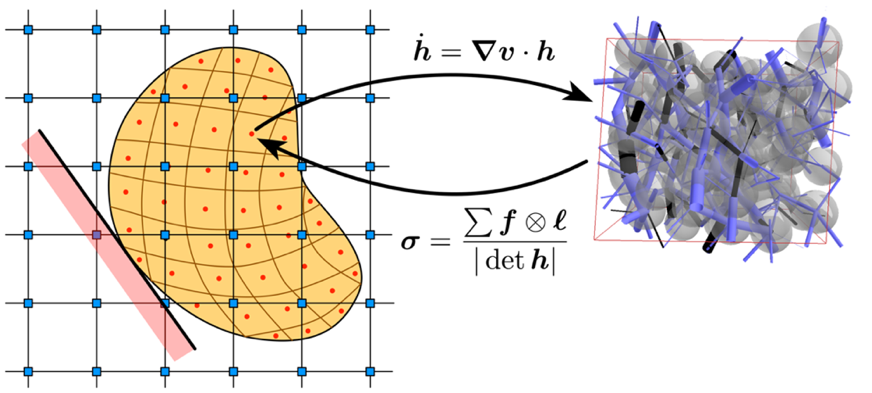
\includegraphics[width=0.5\textwidth]{CouplageMPMxDEM.png}
\caption{Principe d’une approche à deux échelles hiérarchiques~\citep{projetderecherche}.}
\label{fig:MPMxDEM}
\end{figure}

Le couplage entre deux méthodes numériques différentes, comme le couplage FEM$\times$DEM~\citep{nguyen2013modelisation}, a déjà été largement utilisé et s’est avéré très efficace.  
Dans le cadre de la modélisation des écoulements granulaires, le couplage entre la méthode des points matériels (MPM) et la méthode des éléments discrets (DEM) apparaît particulièrement pertinent, car il permet de tirer parti des atouts respectifs de chaque méthode.

Comme illustré sur la \autoref{fig:MPMxDEM}, la méthode MPM (partie gauche) se charge du calcul des indices à l’échelle macroscopique, notamment du gradient de vitesse $\nabla v$. Ces informations sont ensuite transmises aux points matériels rouges, qui sont ici associés à un volume élémentaire représentatif (VER) modélisé par DEM. Ce modèle discret permet de calculer le tenseur des contraintes $\sigma_p$ selon la formulation classique (Love-Weber).

Grâce à l’intégration du modèle DEM au niveau microscopique, il devient possible de résoudre localement les comportements complexes des matériaux, en tenant compte de la microstructure et des interactions entre grains. Cela permet d’aller au-delà des limitations des lois de comportement analytiques classiques, souvent trop simplifiées pour capturer les effets fins liés à la nature granulaire.

Parallèlement, la MPM offre une solution efficace pour représenter le mouvement global du matériau sans souffrir des problèmes de distorsion de maillage, fréquents dans les méthodes lagrangiennes classiques comme la FEM. La combinaison des deux approches permet ainsi de préserver les avantages de chacune tout en compensant leurs faiblesses respectives.

Au laboratoire 3SR, deux programmes de calcul indépendants en \texttt{C++} ont été développés pour implémenter respectivement la MPM et la DEM. Il s'agit de \texttt{MPMbox} pour la MPM, et de \texttt{3D\_sandstone} pour la DEM. Leur intégration dans une plateforme de calcul multi-échelle est désormais bien établie~\citep{richefeu2025mpmxdem}, avec des résultats prometteurs. Toutefois, certains verrous scientifiques restent à résoudre :

\begin{itemize}
    \item \textbf{Équivalence des inerties aux deux échelles:}  
    La méthode MPM, conçue à l’origine pour traiter des problèmes de contact dynamique~\citep{nguyen2023material}, intègre naturellement les effets d’inertie. En revanche, la DEM tend à filtrer les réponses dynamiques en attendant une stabilisation statique~\citep{nguyen2014fem}. Le couplage des deux fait émerger des questions théoriques nouvelles concernant l’équivalence des inerties entre les échelles micro et macro, particulièrement critiques dans les contextes hautement dynamiques comme les écoulements granulaires.

    \item \textbf{Conditions aux limites et conditions initiales:}  
    L’implémentation actuelle des conditions aux limites périodiques dans la partie DEM reste imparfaite. Cette insuffisance engendre parfois des pics anormaux de contraintes, nuisant à la robustesse et à la représentativité des simulations.
\end{itemize}



\chapter{L'étude pratique}

\section{Simulation MPM – Déformation d'une poutre en console}

Afin de valider la justesse de l’implémentation du programme MPM, une poutre en console encastrée, soumise à son propre poids (gravité), a été choisie comme cas test.  
La simulation est d’abord effectuée avec une loi de comportement élastique de Hooke (loi de l’élasticité linéaire), et les résultats numériques sont comparés à la solution analytique issue de la résistance des matériaux.

\begin{figure}[h]
\centering
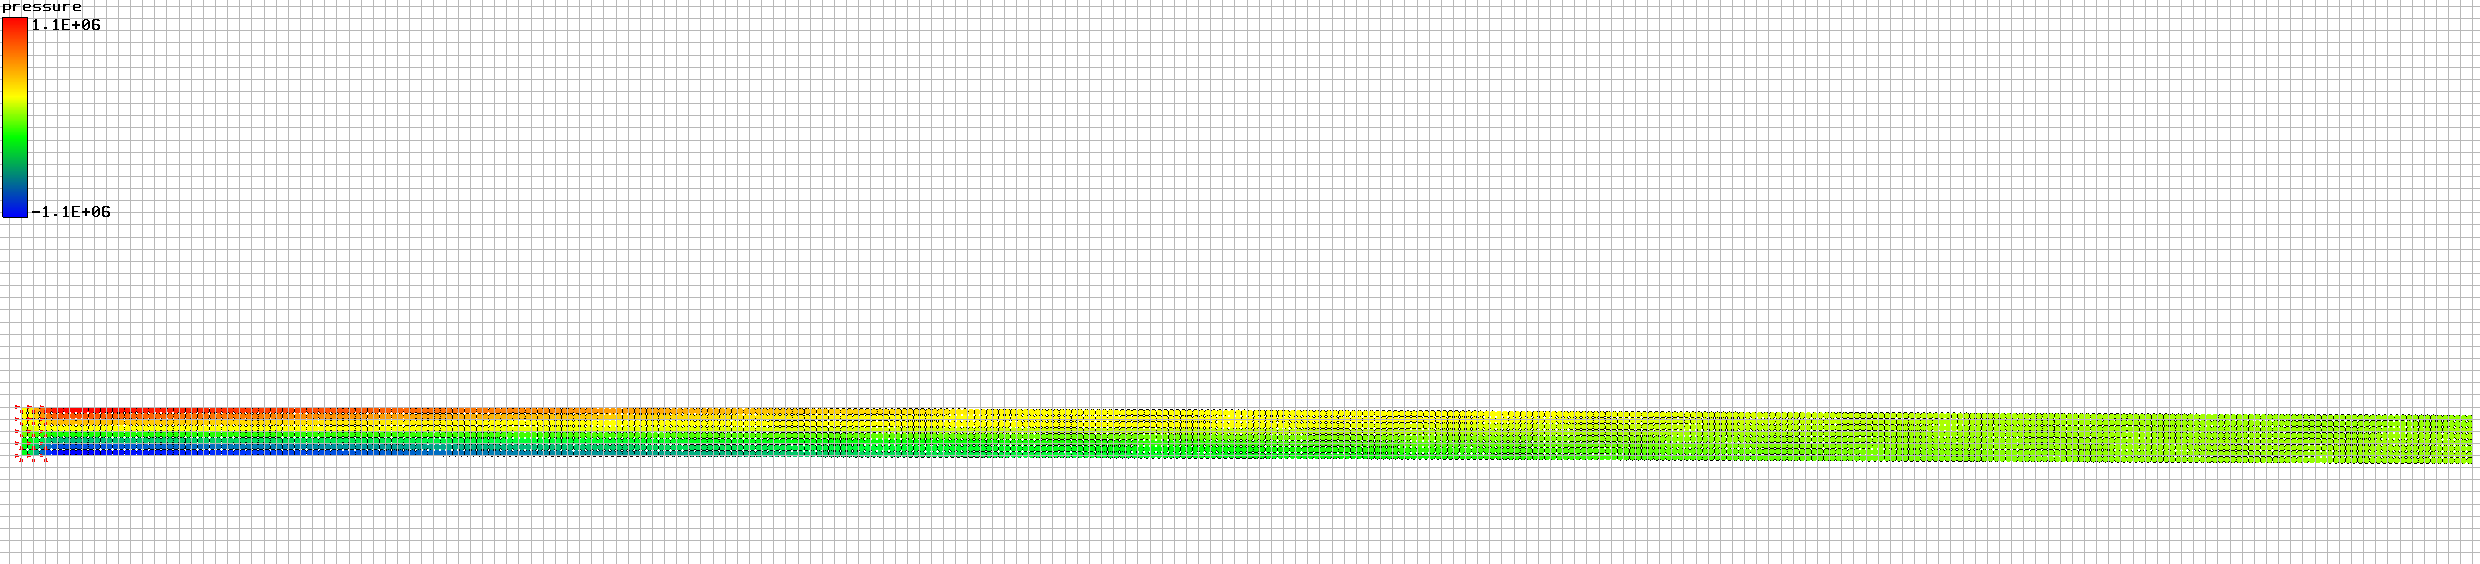
\includegraphics[height=0.13\textheight]{Model_Poutre.png}
\caption{Modèle de poutre encastrée en console}
\label{fig:ModelPoutre}
\end{figure}

\begin{figure}[h]
    \centering
    \small \scalebox{0.6}{% GNUPLOT: LaTeX picture with Postscript
\begingroup
  \makeatletter
  \providecommand\color[2][]{%
    \GenericError{(gnuplot) \space\space\space\@spaces}{%
      Package color not loaded in conjunction with
      terminal option `colourtext'%
    }{See the gnuplot documentation for explanation.%
    }{Either use 'blacktext' in gnuplot or load the package
      color.sty in LaTeX.}%
    \renewcommand\color[2][]{}%
  }%
  \providecommand\includegraphics[2][]{%
    \GenericError{(gnuplot) \space\space\space\@spaces}{%
      Package graphicx or graphics not loaded%
    }{See the gnuplot documentation for explanation.%
    }{The gnuplot epslatex terminal needs graphicx.sty or graphics.sty.}%
    \renewcommand\includegraphics[2][]{}%
  }%
  \providecommand\rotatebox[2]{#2}%
  \@ifundefined{ifGPcolor}{%
    \newif\ifGPcolor
    \GPcolortrue
  }{}%
  \@ifundefined{ifGPblacktext}{%
    \newif\ifGPblacktext
    \GPblacktextfalse
  }{}%
  % define a \g@addto@macro without @ in the name:
  \let\gplgaddtomacro\g@addto@macro
  % define empty templates for all commands taking text:
  \gdef\gplbacktext{}%
  \gdef\gplfronttext{}%
  \makeatother
  \ifGPblacktext
    % no textcolor at all
    \def\colorrgb#1{}%
    \def\colorgray#1{}%
  \else
    % gray or color?
    \ifGPcolor
      \def\colorrgb#1{\color[rgb]{#1}}%
      \def\colorgray#1{\color[gray]{#1}}%
      \expandafter\def\csname LTw\endcsname{\color{white}}%
      \expandafter\def\csname LTb\endcsname{\color{black}}%
      \expandafter\def\csname LTa\endcsname{\color{black}}%
      \expandafter\def\csname LT0\endcsname{\color[rgb]{1,0,0}}%
      \expandafter\def\csname LT1\endcsname{\color[rgb]{0,1,0}}%
      \expandafter\def\csname LT2\endcsname{\color[rgb]{0,0,1}}%
      \expandafter\def\csname LT3\endcsname{\color[rgb]{1,0,1}}%
      \expandafter\def\csname LT4\endcsname{\color[rgb]{0,1,1}}%
      \expandafter\def\csname LT5\endcsname{\color[rgb]{1,1,0}}%
      \expandafter\def\csname LT6\endcsname{\color[rgb]{0,0,0}}%
      \expandafter\def\csname LT7\endcsname{\color[rgb]{1,0.3,0}}%
      \expandafter\def\csname LT8\endcsname{\color[rgb]{0.5,0.5,0.5}}%
    \else
      % gray
      \def\colorrgb#1{\color{black}}%
      \def\colorgray#1{\color[gray]{#1}}%
      \expandafter\def\csname LTw\endcsname{\color{white}}%
      \expandafter\def\csname LTb\endcsname{\color{black}}%
      \expandafter\def\csname LTa\endcsname{\color{black}}%
      \expandafter\def\csname LT0\endcsname{\color{black}}%
      \expandafter\def\csname LT1\endcsname{\color{black}}%
      \expandafter\def\csname LT2\endcsname{\color{black}}%
      \expandafter\def\csname LT3\endcsname{\color{black}}%
      \expandafter\def\csname LT4\endcsname{\color{black}}%
      \expandafter\def\csname LT5\endcsname{\color{black}}%
      \expandafter\def\csname LT6\endcsname{\color{black}}%
      \expandafter\def\csname LT7\endcsname{\color{black}}%
      \expandafter\def\csname LT8\endcsname{\color{black}}%
    \fi
  \fi
    \setlength{\unitlength}{0.0500bp}%
    \ifx\gptboxheight\undefined%
      \newlength{\gptboxheight}%
      \newlength{\gptboxwidth}%
      \newsavebox{\gptboxtext}%
    \fi%
    \setlength{\fboxrule}{0.5pt}%
    \setlength{\fboxsep}{1pt}%
    \definecolor{tbcol}{rgb}{1,1,1}%
\begin{picture}(7200.00,5040.00)%
    \gplgaddtomacro\gplbacktext{%
      \csname LTb\endcsname%%
      \put(682,704){\makebox(0,0)[r]{\strut{}$-5$}}%
      \csname LTb\endcsname%%
      \put(682,1390){\makebox(0,0)[r]{\strut{}$-4$}}%
      \csname LTb\endcsname%%
      \put(682,2076){\makebox(0,0)[r]{\strut{}$-3$}}%
      \csname LTb\endcsname%%
      \put(682,2762){\makebox(0,0)[r]{\strut{}$-2$}}%
      \csname LTb\endcsname%%
      \put(682,3447){\makebox(0,0)[r]{\strut{}$-1$}}%
      \csname LTb\endcsname%%
      \put(682,4133){\makebox(0,0)[r]{\strut{}$0$}}%
      \csname LTb\endcsname%%
      \put(682,4819){\makebox(0,0)[r]{\strut{}$1$}}%
      \csname LTb\endcsname%%
      \put(814,484){\makebox(0,0){\strut{}$0$}}%
      \csname LTb\endcsname%%
      \put(2012,484){\makebox(0,0){\strut{}$0.2$}}%
      \csname LTb\endcsname%%
      \put(3210,484){\makebox(0,0){\strut{}$0.4$}}%
      \csname LTb\endcsname%%
      \put(4407,484){\makebox(0,0){\strut{}$0.6$}}%
      \csname LTb\endcsname%%
      \put(5605,484){\makebox(0,0){\strut{}$0.8$}}%
      \csname LTb\endcsname%%
      \put(6803,484){\makebox(0,0){\strut{}$1$}}%
    }%
    \gplgaddtomacro\gplfronttext{%
      \csname LTb\endcsname%%
      \put(209,2761){\rotatebox{-270}{\makebox(0,0){\strut{}$f_y$ (mm)}}}%
      \put(3808,154){\makebox(0,0){\strut{}$x$ (m)}}%
      \csname LTb\endcsname%%
      \put(6009,4493){\makebox(0,0)[r]{\strut{}$\text{f}_{\text{calcul}}$}}%
      \csname LTb\endcsname%%
      \put(6009,4373){\makebox(0,0)[r]{\strut{}$\text{f}_{\text{théorique}}$}}%
      \csname LTb\endcsname%%
      \put(3808,33733){\makebox(0,0){\strut{}}}%
    }%
    \gplbacktext
    \put(0,0){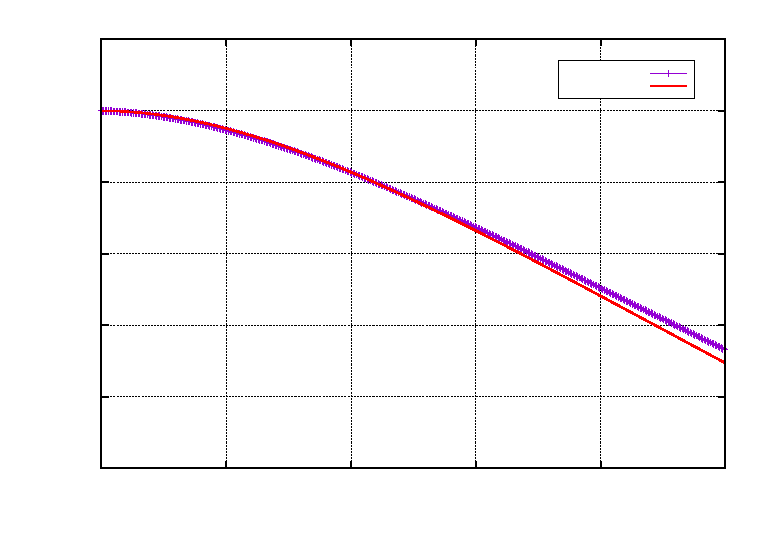
\includegraphics[width={360.00bp},height={252.00bp}]{./Deplacement_Poutre}}%
    \gplfronttext
  \end{picture}%
\endgroup
}
    \caption{Déplacement de la poutre selon l’axe vertical (Y).}
    \label{fig:deplacementPoutre}
\end{figure}

La flèche $f$ de la poutre est donnée par l'expression analytique suivante :

\begin{equation}
    f(x) = \dfrac{-qx^2}{24EI} \times (x^2 - 4Lx + 6L^2)
    \label{eq:fleche}
\end{equation}

où :
$q$ est la charge uniformément répartie sur la longueur de la poutre (en N/m),
$x$ est la position le long de la poutre (en m),
$E$ est le module de Young (en Pa),
$I$ est le moment d'inertie (en m\textsuperscript{4}),
$L$ est la longueur totale de la poutre.

On observe que la déformation obtenue par simulation numérique MPM est en bon accord avec la flèche calculée analytiquement selon l’équation \eqref{eq:fleche}, comme le montre la figure~\ref{fig:deplacementPoutre}.

Il est important de souligner que la longueur d'encastrement ainsi que la discrétisation du maillage dans le cadre de la MPM doivent être soigneusement ajustées à l’échelle géométrique du modèle étudié pour garantir une précision optimale.


%\subsection{Étude sur le cas dynamique}



\section{Simulation DEM: Compression triaxiale}

\begin{figure}[h]
    \centering
    \animategraphics[loop,autoplay,width=5cm]{10}{Triaxial_}{1}{8}
    \caption{Déformation de l’échantillon dans la cellule triaxiale}
    \label{fig:boiteDeformation}
\end{figure}

Dans cette section, nous réalisons une simulation de compression triaxial à l’aide de la méthode DEM, qui comprend deux étapes principales :

\begin{itemize}
    \item \textbf{Préparation de l’échantillon:}  
    Un échantillon est constitué d’un boîtier contenant des particules sphériques non cohésives représentant du sable sec. Ces particules sont générées aléatoirement. Un processus de compression isotrope est ensuite appliqué, avec différentes valeurs du coefficient de frottement  $\mu$ variant de 0 à 1.  
    Cette étape permet de créer des échantillons de densités différentes (plus ou moins compactés), selon l’évolution du paramètre $\mu$.

    \item \textbf{Compression triaxiale:}  
    L’échantillon préparé est ensuite soumis à une contrainte de confinement constant  selon les directions $x$ et $z$ (i.e. $\sigma_{xx} = \sigma_{zz}$). Une déformation axiale contrôlé  est imposée selon l’axe vertical $y$ — illustrée à la figure~\ref{fig:boiteDeformation}.  
    Une première série de simulations est menée en compactant lentement l’échantillon, afin d’analyser l’effet des conditions initiales (structure de l’échantillon) sur la réponse mécanique macroscopique.

    Ensuite, dans la perspective d’une intégration au couplage MPM$\times$DEM, une seconde étude est réalisée en augmentant la vitesse de déformation. Cela permet d’examiner l’influence du nombre l'inertie sur la réponse du matériau, en explorant une large gamme du nombre d’inerti  $I$ (de $10^{-6}$ à $10^{-2}$).
\end{itemize}

% \begin{table}[h]
% \centering
% \begin{tabular}{|c|c|c|c|}
% \hline
% \textbf{Symbole} & \textbf{Paramètre} & \textbf{Valeurs} & \textbf{Unité} \\ 
% \hline
% Nombre de particules & $N$ & $15^3$ & $-$ \\  
% \hline
% Rayon des particules & $R$ & 0.003 $\div$ 0.005 & m \\  
% \hline
% Masse volumique & $\rho$ & 2500 & kg/m$^3$ \\
% \hline
% Contraintes de confinement & $\sigma_{xx} = \sigma_{zz}$ & 100, 200, 300 & kPa \\ 
% \hline
% Raideur normale et tangentielle & $k_n$ \& $k_t$ & $10^6$, $2 \times 10^6$, $3 \times 10^6$ & N/m \\ 
% \hline
% Niveau de raideur (sans dimension) & $\kappa$ & 1000 & $-$ \\ 
% \hline
% Coefficient de frottement & $\mu$ & 0.5 & $-$ \\ 
% \hline
% Déformation axiale maximale & $\varepsilon_{\text{yy}}$ &  80 & \% \\ 
% \hline
% Nombre d’inertie & $I$ & $10^{-6} \div 10^{-2}$ & $-$ \\ 
% \hline
% Pas de temps & $d_t$ & $10^{-6} \div 10^{-10}$ & s \\
% \hline
% \end{tabular}
% \caption{Paramètres utilisés pour la simulation de compression triaxiale}
% \label{tab:parametre}
% \end{table}


\subsection{Les caractéristiques mécaniques générales du sol}

\subsubsection{Étude paramétrique sur la fraction solide}

La fraction solide caractérise la dispersion des particules solides $V_s$ dans un volume $V$.  
C'est un indice important en rhéologie de l'écoulement.  
\begin{equation}
\Phi = \dfrac{V_s}{V} = \dfrac{\sum\limits_{i=1}^n \frac{4}{3}\pi R_i^3}{\det(h)}
\end{equation}

\begin{figure}[h!]
    \centering
    \small
    \scalebox{0.5}{% GNUPLOT: LaTeX picture with Postscript
\begingroup
  \makeatletter
  \providecommand\color[2][]{%
    \GenericError{(gnuplot) \space\space\space\@spaces}{%
      Package color not loaded in conjunction with
      terminal option `colourtext'%
    }{See the gnuplot documentation for explanation.%
    }{Either use 'blacktext' in gnuplot or load the package
      color.sty in LaTeX.}%
    \renewcommand\color[2][]{}%
  }%
  \providecommand\includegraphics[2][]{%
    \GenericError{(gnuplot) \space\space\space\@spaces}{%
      Package graphicx or graphics not loaded%
    }{See the gnuplot documentation for explanation.%
    }{The gnuplot epslatex terminal needs graphicx.sty or graphics.sty.}%
    \renewcommand\includegraphics[2][]{}%
  }%
  \providecommand\rotatebox[2]{#2}%
  \@ifundefined{ifGPcolor}{%
    \newif\ifGPcolor
    \GPcolortrue
  }{}%
  \@ifundefined{ifGPblacktext}{%
    \newif\ifGPblacktext
    \GPblacktextfalse
  }{}%
  % define a \g@addto@macro without @ in the name:
  \let\gplgaddtomacro\g@addto@macro
  % define empty templates for all commands taking text:
  \gdef\gplbacktext{}%
  \gdef\gplfronttext{}%
  \makeatother
  \ifGPblacktext
    % no textcolor at all
    \def\colorrgb#1{}%
    \def\colorgray#1{}%
  \else
    % gray or color?
    \ifGPcolor
      \def\colorrgb#1{\color[rgb]{#1}}%
      \def\colorgray#1{\color[gray]{#1}}%
      \expandafter\def\csname LTw\endcsname{\color{white}}%
      \expandafter\def\csname LTb\endcsname{\color{black}}%
      \expandafter\def\csname LTa\endcsname{\color{black}}%
      \expandafter\def\csname LT0\endcsname{\color[rgb]{1,0,0}}%
      \expandafter\def\csname LT1\endcsname{\color[rgb]{0,1,0}}%
      \expandafter\def\csname LT2\endcsname{\color[rgb]{0,0,1}}%
      \expandafter\def\csname LT3\endcsname{\color[rgb]{1,0,1}}%
      \expandafter\def\csname LT4\endcsname{\color[rgb]{0,1,1}}%
      \expandafter\def\csname LT5\endcsname{\color[rgb]{1,1,0}}%
      \expandafter\def\csname LT6\endcsname{\color[rgb]{0,0,0}}%
      \expandafter\def\csname LT7\endcsname{\color[rgb]{1,0.3,0}}%
      \expandafter\def\csname LT8\endcsname{\color[rgb]{0.5,0.5,0.5}}%
    \else
      % gray
      \def\colorrgb#1{\color{black}}%
      \def\colorgray#1{\color[gray]{#1}}%
      \expandafter\def\csname LTw\endcsname{\color{white}}%
      \expandafter\def\csname LTb\endcsname{\color{black}}%
      \expandafter\def\csname LTa\endcsname{\color{black}}%
      \expandafter\def\csname LT0\endcsname{\color{black}}%
      \expandafter\def\csname LT1\endcsname{\color{black}}%
      \expandafter\def\csname LT2\endcsname{\color{black}}%
      \expandafter\def\csname LT3\endcsname{\color{black}}%
      \expandafter\def\csname LT4\endcsname{\color{black}}%
      \expandafter\def\csname LT5\endcsname{\color{black}}%
      \expandafter\def\csname LT6\endcsname{\color{black}}%
      \expandafter\def\csname LT7\endcsname{\color{black}}%
      \expandafter\def\csname LT8\endcsname{\color{black}}%
    \fi
  \fi
    \setlength{\unitlength}{0.0500bp}%
    \ifx\gptboxheight\undefined%
      \newlength{\gptboxheight}%
      \newlength{\gptboxwidth}%
      \newsavebox{\gptboxtext}%
    \fi%
    \setlength{\fboxrule}{0.5pt}%
    \setlength{\fboxsep}{1pt}%
    \definecolor{tbcol}{rgb}{1,1,1}%
\begin{picture}(7200.00,5040.00)%
    \gplgaddtomacro\gplbacktext{%
      \csname LTb\endcsname%%
      \put(946,704){\makebox(0,0)[r]{\strut{}$0.56$}}%
      \csname LTb\endcsname%%
      \put(946,1218){\makebox(0,0)[r]{\strut{}$0.57$}}%
      \csname LTb\endcsname%%
      \put(946,1733){\makebox(0,0)[r]{\strut{}$0.58$}}%
      \csname LTb\endcsname%%
      \put(946,2247){\makebox(0,0)[r]{\strut{}$0.59$}}%
      \csname LTb\endcsname%%
      \put(946,2762){\makebox(0,0)[r]{\strut{}$0.6$}}%
      \csname LTb\endcsname%%
      \put(946,3276){\makebox(0,0)[r]{\strut{}$0.61$}}%
      \csname LTb\endcsname%%
      \put(946,3790){\makebox(0,0)[r]{\strut{}$0.62$}}%
      \csname LTb\endcsname%%
      \put(946,4305){\makebox(0,0)[r]{\strut{}$0.63$}}%
      \csname LTb\endcsname%%
      \put(946,4819){\makebox(0,0)[r]{\strut{}$0.64$}}%
      \csname LTb\endcsname%%
      \put(1598,484){\makebox(0,0){\strut{}$0.1$}}%
      \csname LTb\endcsname%%
      \put(2177,484){\makebox(0,0){\strut{}$0.2$}}%
      \csname LTb\endcsname%%
      \put(2755,484){\makebox(0,0){\strut{}$0.3$}}%
      \csname LTb\endcsname%%
      \put(3333,484){\makebox(0,0){\strut{}$0.4$}}%
      \csname LTb\endcsname%%
      \put(3912,484){\makebox(0,0){\strut{}$0.5$}}%
      \csname LTb\endcsname%%
      \put(4490,484){\makebox(0,0){\strut{}$0.6$}}%
      \csname LTb\endcsname%%
      \put(5068,484){\makebox(0,0){\strut{}$0.7$}}%
      \csname LTb\endcsname%%
      \put(5646,484){\makebox(0,0){\strut{}$0.8$}}%
      \csname LTb\endcsname%%
      \put(6225,484){\makebox(0,0){\strut{}$0.9$}}%
      \csname LTb\endcsname%%
      \put(6803,484){\makebox(0,0){\strut{}$1$}}%
    }%
    \gplgaddtomacro\gplfronttext{%
      \csname LTb\endcsname%%
      \put(209,2761){\rotatebox{-270}{\makebox(0,0){\strut{}$\Phi$}}}%
      \put(3940,154){\makebox(0,0){\strut{}$\mu$}}%
      \csname LTb\endcsname%%
      \put(3940,26625){\makebox(0,0){\strut{}}}%
    }%
    \gplbacktext
    \put(0,0){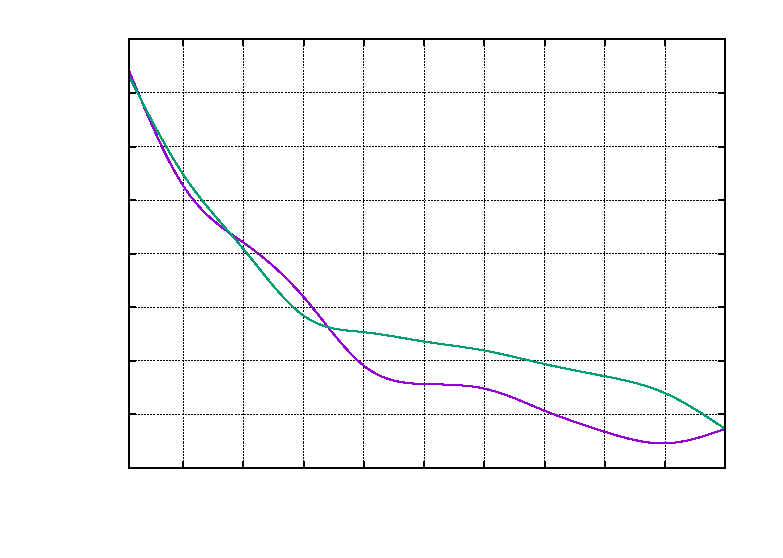
\includegraphics[width={360.00bp},height={252.00bp}]{./fractonSolide}}%
    \gplfronttext
  \end{picture}%
\endgroup
}
    \caption{La fraction solide}
    \label{fig:fractionSolideMax}
\end{figure}

La \autoref{fig:fractionSolideMax} montre que la valeur maximale $\Phi_{\max}$ pour une dispersion désordonnée de sphères en contact dense est approximativement égale à 0.64~\citep{combe2023demlecture}.  

Un point important est que le paramètre $\mu$ augmente de 0 à 1 lors de la préparation des échantillons. Ceci correspond à une diminution progressive de la densité apparente, ce qui est confirmé par le graphique. En effet, plus $\mu$ est élevé, plus l’arrangement des grains devient difficile à organiser.

\subsubsection{Comportement général des échantillons et état critique}

On peut exprimer le rapport $q/p$ par la relation suivante :
\begin{equation}
\frac{q}{p} \approx \frac{\sigma_{yy} - \frac{1}{2}(\sigma_{xx} + \sigma_{zz})}{\frac{1}{2}(\sigma_{xx} + \sigma_{zz})}
\label{eq:qformulation}
\end{equation}

\begin{figure}[htbp]
    \centering
    \begin{subfigure}[b]{0.49\textwidth}
        \centering
        \small
        \scalebox{0.5}{% GNUPLOT: LaTeX picture with Postscript
\begingroup
  \makeatletter
  \providecommand\color[2][]{%
    \GenericError{(gnuplot) \space\space\space\@spaces}{%
      Package color not loaded in conjunction with
      terminal option `colourtext'%
    }{See the gnuplot documentation for explanation.%
    }{Either use 'blacktext' in gnuplot or load the package
      color.sty in LaTeX.}%
    \renewcommand\color[2][]{}%
  }%
  \providecommand\includegraphics[2][]{%
    \GenericError{(gnuplot) \space\space\space\@spaces}{%
      Package graphicx or graphics not loaded%
    }{See the gnuplot documentation for explanation.%
    }{The gnuplot epslatex terminal needs graphicx.sty or graphics.sty.}%
    \renewcommand\includegraphics[2][]{}%
  }%
  \providecommand\rotatebox[2]{#2}%
  \@ifundefined{ifGPcolor}{%
    \newif\ifGPcolor
    \GPcolortrue
  }{}%
  \@ifundefined{ifGPblacktext}{%
    \newif\ifGPblacktext
    \GPblacktexttrue
  }{}%
  % define a \g@addto@macro without @ in the name:
  \let\gplgaddtomacro\g@addto@macro
  % define empty templates for all commands taking text:
  \gdef\gplbacktext{}%
  \gdef\gplfronttext{}%
  \makeatother
  \ifGPblacktext
    % no textcolor at all
    \def\colorrgb#1{}%
    \def\colorgray#1{}%
  \else
    % gray or color?
    \ifGPcolor
      \def\colorrgb#1{\color[rgb]{#1}}%
      \def\colorgray#1{\color[gray]{#1}}%
      \expandafter\def\csname LTw\endcsname{\color{white}}%
      \expandafter\def\csname LTb\endcsname{\color{black}}%
      \expandafter\def\csname LTa\endcsname{\color{black}}%
      \expandafter\def\csname LT0\endcsname{\color[rgb]{1,0,0}}%
      \expandafter\def\csname LT1\endcsname{\color[rgb]{0,1,0}}%
      \expandafter\def\csname LT2\endcsname{\color[rgb]{0,0,1}}%
      \expandafter\def\csname LT3\endcsname{\color[rgb]{1,0,1}}%
      \expandafter\def\csname LT4\endcsname{\color[rgb]{0,1,1}}%
      \expandafter\def\csname LT5\endcsname{\color[rgb]{1,1,0}}%
      \expandafter\def\csname LT6\endcsname{\color[rgb]{0,0,0}}%
      \expandafter\def\csname LT7\endcsname{\color[rgb]{1,0.3,0}}%
      \expandafter\def\csname LT8\endcsname{\color[rgb]{0.5,0.5,0.5}}%
    \else
      % gray
      \def\colorrgb#1{\color{black}}%
      \def\colorgray#1{\color[gray]{#1}}%
      \expandafter\def\csname LTw\endcsname{\color{white}}%
      \expandafter\def\csname LTb\endcsname{\color{black}}%
      \expandafter\def\csname LTa\endcsname{\color{black}}%
      \expandafter\def\csname LT0\endcsname{\color{black}}%
      \expandafter\def\csname LT1\endcsname{\color{black}}%
      \expandafter\def\csname LT2\endcsname{\color{black}}%
      \expandafter\def\csname LT3\endcsname{\color{black}}%
      \expandafter\def\csname LT4\endcsname{\color{black}}%
      \expandafter\def\csname LT5\endcsname{\color{black}}%
      \expandafter\def\csname LT6\endcsname{\color{black}}%
      \expandafter\def\csname LT7\endcsname{\color{black}}%
      \expandafter\def\csname LT8\endcsname{\color{black}}%
    \fi
  \fi
    \setlength{\unitlength}{0.0500bp}%
    \ifx\gptboxheight\undefined%
      \newlength{\gptboxheight}%
      \newlength{\gptboxwidth}%
      \newsavebox{\gptboxtext}%
    \fi%
    \setlength{\fboxrule}{0.5pt}%
    \setlength{\fboxsep}{1pt}%
    \definecolor{tbcol}{rgb}{1,1,1}%
\begin{picture}(7200.00,5040.00)%
    \gplgaddtomacro\gplbacktext{%
      \csname LTb\endcsname%%
      \put(946,704){\makebox(0,0)[r]{\strut{}$-0.5$}}%
      \csname LTb\endcsname%%
      \put(946,1390){\makebox(0,0)[r]{\strut{}$0$}}%
      \csname LTb\endcsname%%
      \put(946,2076){\makebox(0,0)[r]{\strut{}$0.5$}}%
      \csname LTb\endcsname%%
      \put(946,2762){\makebox(0,0)[r]{\strut{}$1$}}%
      \csname LTb\endcsname%%
      \put(946,3447){\makebox(0,0)[r]{\strut{}$1.5$}}%
      \csname LTb\endcsname%%
      \put(946,4133){\makebox(0,0)[r]{\strut{}$2$}}%
      \csname LTb\endcsname%%
      \put(946,4819){\makebox(0,0)[r]{\strut{}$2.5$}}%
      \csname LTb\endcsname%%
      \put(1078,484){\makebox(0,0){\strut{}$0$}}%
      \csname LTb\endcsname%%
      \put(2223,484){\makebox(0,0){\strut{}$2$}}%
      \csname LTb\endcsname%%
      \put(3368,484){\makebox(0,0){\strut{}$4$}}%
      \csname LTb\endcsname%%
      \put(4513,484){\makebox(0,0){\strut{}$6$}}%
      \csname LTb\endcsname%%
      \put(5658,484){\makebox(0,0){\strut{}$8$}}%
      \csname LTb\endcsname%%
      \put(6803,484){\makebox(0,0){\strut{}$10$}}%
    }%
    \gplgaddtomacro\gplfronttext{%
      \csname LTb\endcsname%%
      \put(209,2761){\rotatebox{-270}{\makebox(0,0){\strut{}$\frac{q}{\sigma_0}$}}}%
      \put(3940,154){\makebox(0,0){\strut{}$\varepsilon_{yy}$ (\%)}}%
      \csname LTb\endcsname%%
      \put(5960,2288){\makebox(0,0)[r]{\strut{}$\mu = 0$}}%
      \csname LTb\endcsname%%
      \put(5960,2054){\makebox(0,0)[r]{\strut{}$\mu = 0.1$}}%
      \csname LTb\endcsname%%
      \put(5960,1820){\makebox(0,0)[r]{\strut{}$\mu = 0.2$}}%
      \csname LTb\endcsname%%
      \put(5960,1586){\makebox(0,0)[r]{\strut{}$\mu = 0.3$}}%
      \csname LTb\endcsname%%
      \put(5960,1352){\makebox(0,0)[r]{\strut{}$\mu = 0.4$}}%
      \csname LTb\endcsname%%
      \put(5960,1118){\makebox(0,0)[r]{\strut{}$\mu = 0.45$}}%
      \csname LTb\endcsname%%
      \put(5960,884){\makebox(0,0)[r]{\strut{}$\mu = 0.5$}}%
    }%
    \gplbacktext
    \put(0,0){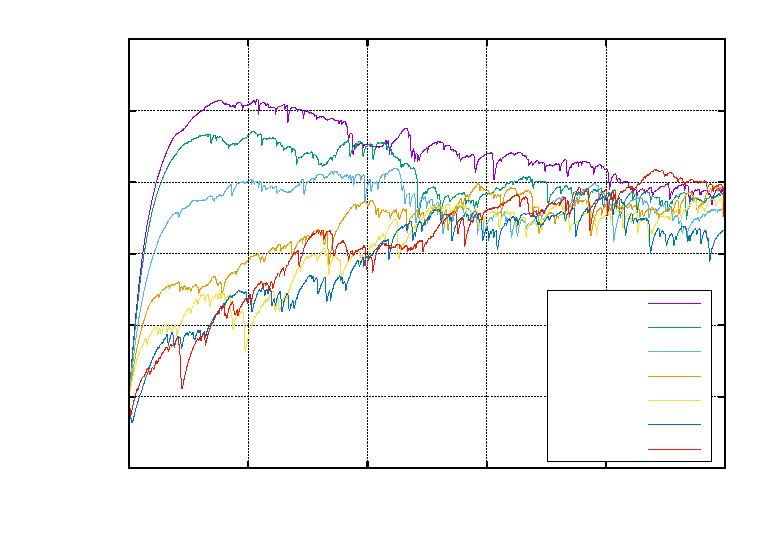
\includegraphics[width={360.00bp},height={252.00bp}]{./Contrainte-Deformation}}%
    \gplfronttext
  \end{picture}%
\endgroup
}
        \caption{Contrainte-Déformation}
        \label{fig:contrainte}
    \end{subfigure}
    \hfill
    \begin{subfigure}[b]{0.49\textwidth}
        \centering
        \small
        \scalebox{0.5}{% GNUPLOT: LaTeX picture with Postscript
\begingroup
  \makeatletter
  \providecommand\color[2][]{%
    \GenericError{(gnuplot) \space\space\space\@spaces}{%
      Package color not loaded in conjunction with
      terminal option `colourtext'%
    }{See the gnuplot documentation for explanation.%
    }{Either use 'blacktext' in gnuplot or load the package
      color.sty in LaTeX.}%
    \renewcommand\color[2][]{}%
  }%
  \providecommand\includegraphics[2][]{%
    \GenericError{(gnuplot) \space\space\space\@spaces}{%
      Package graphicx or graphics not loaded%
    }{See the gnuplot documentation for explanation.%
    }{The gnuplot epslatex terminal needs graphicx.sty or graphics.sty.}%
    \renewcommand\includegraphics[2][]{}%
  }%
  \providecommand\rotatebox[2]{#2}%
  \@ifundefined{ifGPcolor}{%
    \newif\ifGPcolor
    \GPcolortrue
  }{}%
  \@ifundefined{ifGPblacktext}{%
    \newif\ifGPblacktext
    \GPblacktexttrue
  }{}%
  % define a \g@addto@macro without @ in the name:
  \let\gplgaddtomacro\g@addto@macro
  % define empty templates for all commands taking text:
  \gdef\gplbacktext{}%
  \gdef\gplfronttext{}%
  \makeatother
  \ifGPblacktext
    % no textcolor at all
    \def\colorrgb#1{}%
    \def\colorgray#1{}%
  \else
    % gray or color?
    \ifGPcolor
      \def\colorrgb#1{\color[rgb]{#1}}%
      \def\colorgray#1{\color[gray]{#1}}%
      \expandafter\def\csname LTw\endcsname{\color{white}}%
      \expandafter\def\csname LTb\endcsname{\color{black}}%
      \expandafter\def\csname LTa\endcsname{\color{black}}%
      \expandafter\def\csname LT0\endcsname{\color[rgb]{1,0,0}}%
      \expandafter\def\csname LT1\endcsname{\color[rgb]{0,1,0}}%
      \expandafter\def\csname LT2\endcsname{\color[rgb]{0,0,1}}%
      \expandafter\def\csname LT3\endcsname{\color[rgb]{1,0,1}}%
      \expandafter\def\csname LT4\endcsname{\color[rgb]{0,1,1}}%
      \expandafter\def\csname LT5\endcsname{\color[rgb]{1,1,0}}%
      \expandafter\def\csname LT6\endcsname{\color[rgb]{0,0,0}}%
      \expandafter\def\csname LT7\endcsname{\color[rgb]{1,0.3,0}}%
      \expandafter\def\csname LT8\endcsname{\color[rgb]{0.5,0.5,0.5}}%
    \else
      % gray
      \def\colorrgb#1{\color{black}}%
      \def\colorgray#1{\color[gray]{#1}}%
      \expandafter\def\csname LTw\endcsname{\color{white}}%
      \expandafter\def\csname LTb\endcsname{\color{black}}%
      \expandafter\def\csname LTa\endcsname{\color{black}}%
      \expandafter\def\csname LT0\endcsname{\color{black}}%
      \expandafter\def\csname LT1\endcsname{\color{black}}%
      \expandafter\def\csname LT2\endcsname{\color{black}}%
      \expandafter\def\csname LT3\endcsname{\color{black}}%
      \expandafter\def\csname LT4\endcsname{\color{black}}%
      \expandafter\def\csname LT5\endcsname{\color{black}}%
      \expandafter\def\csname LT6\endcsname{\color{black}}%
      \expandafter\def\csname LT7\endcsname{\color{black}}%
      \expandafter\def\csname LT8\endcsname{\color{black}}%
    \fi
  \fi
    \setlength{\unitlength}{0.0500bp}%
    \ifx\gptboxheight\undefined%
      \newlength{\gptboxheight}%
      \newlength{\gptboxwidth}%
      \newsavebox{\gptboxtext}%
    \fi%
    \setlength{\fboxrule}{0.5pt}%
    \setlength{\fboxsep}{1pt}%
    \definecolor{tbcol}{rgb}{1,1,1}%
\begin{picture}(7200.00,5040.00)%
    \gplgaddtomacro\gplbacktext{%
      \csname LTb\endcsname%%
      \put(682,704){\makebox(0,0)[r]{\strut{}$-4$}}%
      \csname LTb\endcsname%%
      \put(682,1161){\makebox(0,0)[r]{\strut{}$-3$}}%
      \csname LTb\endcsname%%
      \put(682,1618){\makebox(0,0)[r]{\strut{}$-2$}}%
      \csname LTb\endcsname%%
      \put(682,2076){\makebox(0,0)[r]{\strut{}$-1$}}%
      \csname LTb\endcsname%%
      \put(682,2533){\makebox(0,0)[r]{\strut{}$0$}}%
      \csname LTb\endcsname%%
      \put(682,2990){\makebox(0,0)[r]{\strut{}$1$}}%
      \csname LTb\endcsname%%
      \put(682,3447){\makebox(0,0)[r]{\strut{}$2$}}%
      \csname LTb\endcsname%%
      \put(682,3905){\makebox(0,0)[r]{\strut{}$3$}}%
      \csname LTb\endcsname%%
      \put(682,4362){\makebox(0,0)[r]{\strut{}$4$}}%
      \csname LTb\endcsname%%
      \put(682,4819){\makebox(0,0)[r]{\strut{}$5$}}%
      \csname LTb\endcsname%%
      \put(814,484){\makebox(0,0){\strut{}$0$}}%
      \csname LTb\endcsname%%
      \put(2012,484){\makebox(0,0){\strut{}$2$}}%
      \csname LTb\endcsname%%
      \put(3210,484){\makebox(0,0){\strut{}$4$}}%
      \csname LTb\endcsname%%
      \put(4407,484){\makebox(0,0){\strut{}$6$}}%
      \csname LTb\endcsname%%
      \put(5605,484){\makebox(0,0){\strut{}$8$}}%
      \csname LTb\endcsname%%
      \put(6803,484){\makebox(0,0){\strut{}$10$}}%
    }%
    \gplgaddtomacro\gplfronttext{%
      \csname LTb\endcsname%%
      \put(209,2761){\rotatebox{-270}{\makebox(0,0){\strut{}$\varepsilon_{v}$ (\%)}}}%
      \put(3808,154){\makebox(0,0){\strut{}$\varepsilon_{yy}$ (\%)}}%
      \csname LTb\endcsname%%
      \put(1810,4639){\makebox(0,0)[r]{\strut{}$\mu = 0$}}%
      \csname LTb\endcsname%%
      \put(1810,4405){\makebox(0,0)[r]{\strut{}$\mu = 0.1$}}%
      \csname LTb\endcsname%%
      \put(1810,4171){\makebox(0,0)[r]{\strut{}$\mu = 0.2$}}%
      \csname LTb\endcsname%%
      \put(1810,3937){\makebox(0,0)[r]{\strut{}$\mu = 0.3$}}%
      \csname LTb\endcsname%%
      \put(1810,3703){\makebox(0,0)[r]{\strut{}$\mu = 0.4$}}%
      \csname LTb\endcsname%%
      \put(1810,3469){\makebox(0,0)[r]{\strut{}$\mu = 0.45$}}%
      \csname LTb\endcsname%%
      \put(1810,3235){\makebox(0,0)[r]{\strut{}$\mu = 0.5$}}%
    }%
    \gplbacktext
    \put(0,0){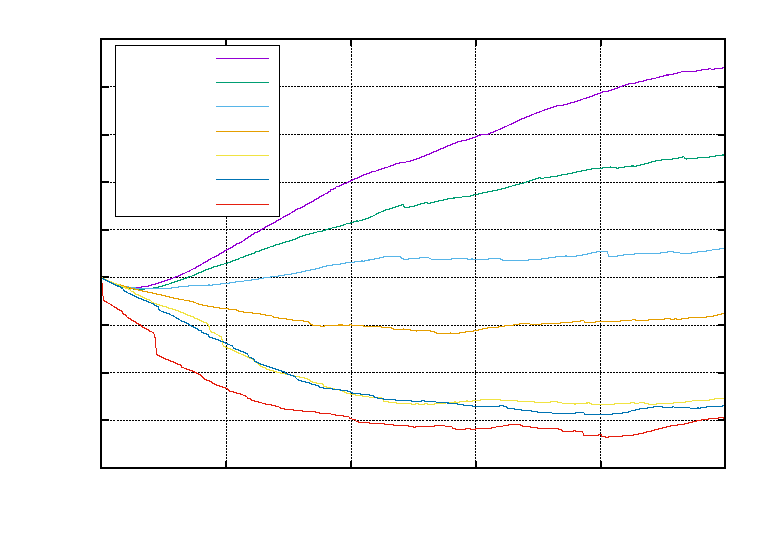
\includegraphics[width={360.00bp},height={252.00bp}]{./Deformation_Volumique}}%
    \gplfronttext
  \end{picture}%
\endgroup
}
        \caption{Déformation volumique}
        \label{fig:defvo}
    \end{subfigure}
    \caption{Réponses macroscopiques des essais triaxiaux lents}
    \label{fig:comparaison}
\end{figure}

\begin{figure}[h!]
    \centering
    \subfloat[Norme des forces]{\scalebox{0.33}{\small % GNUPLOT: LaTeX picture with Postscript
\begingroup
  \makeatletter
  \providecommand\color[2][]{%
    \GenericError{(gnuplot) \space\space\space\@spaces}{%
      Package color not loaded in conjunction with
      terminal option `colourtext'%
    }{See the gnuplot documentation for explanation.%
    }{Either use 'blacktext' in gnuplot or load the package
      color.sty in LaTeX.}%
    \renewcommand\color[2][]{}%
  }%
  \providecommand\includegraphics[2][]{%
    \GenericError{(gnuplot) \space\space\space\@spaces}{%
      Package graphicx or graphics not loaded%
    }{See the gnuplot documentation for explanation.%
    }{The gnuplot epslatex terminal needs graphicx.sty or graphics.sty.}%
    \renewcommand\includegraphics[2][]{}%
  }%
  \providecommand\rotatebox[2]{#2}%
  \@ifundefined{ifGPcolor}{%
    \newif\ifGPcolor
    \GPcolortrue
  }{}%
  \@ifundefined{ifGPblacktext}{%
    \newif\ifGPblacktext
    \GPblacktexttrue
  }{}%
  % define a \g@addto@macro without @ in the name:
  \let\gplgaddtomacro\g@addto@macro
  % define empty templates for all commands taking text:
  \gdef\gplbacktext{}%
  \gdef\gplfronttext{}%
  \makeatother
  \ifGPblacktext
    % no textcolor at all
    \def\colorrgb#1{}%
    \def\colorgray#1{}%
  \else
    % gray or color?
    \ifGPcolor
      \def\colorrgb#1{\color[rgb]{#1}}%
      \def\colorgray#1{\color[gray]{#1}}%
      \expandafter\def\csname LTw\endcsname{\color{white}}%
      \expandafter\def\csname LTb\endcsname{\color{black}}%
      \expandafter\def\csname LTa\endcsname{\color{black}}%
      \expandafter\def\csname LT0\endcsname{\color[rgb]{1,0,0}}%
      \expandafter\def\csname LT1\endcsname{\color[rgb]{0,1,0}}%
      \expandafter\def\csname LT2\endcsname{\color[rgb]{0,0,1}}%
      \expandafter\def\csname LT3\endcsname{\color[rgb]{1,0,1}}%
      \expandafter\def\csname LT4\endcsname{\color[rgb]{0,1,1}}%
      \expandafter\def\csname LT5\endcsname{\color[rgb]{1,1,0}}%
      \expandafter\def\csname LT6\endcsname{\color[rgb]{0,0,0}}%
      \expandafter\def\csname LT7\endcsname{\color[rgb]{1,0.3,0}}%
      \expandafter\def\csname LT8\endcsname{\color[rgb]{0.5,0.5,0.5}}%
    \else
      % gray
      \def\colorrgb#1{\color{black}}%
      \def\colorgray#1{\color[gray]{#1}}%
      \expandafter\def\csname LTw\endcsname{\color{white}}%
      \expandafter\def\csname LTb\endcsname{\color{black}}%
      \expandafter\def\csname LTa\endcsname{\color{black}}%
      \expandafter\def\csname LT0\endcsname{\color{black}}%
      \expandafter\def\csname LT1\endcsname{\color{black}}%
      \expandafter\def\csname LT2\endcsname{\color{black}}%
      \expandafter\def\csname LT3\endcsname{\color{black}}%
      \expandafter\def\csname LT4\endcsname{\color{black}}%
      \expandafter\def\csname LT5\endcsname{\color{black}}%
      \expandafter\def\csname LT6\endcsname{\color{black}}%
      \expandafter\def\csname LT7\endcsname{\color{black}}%
      \expandafter\def\csname LT8\endcsname{\color{black}}%
    \fi
  \fi
    \setlength{\unitlength}{0.0500bp}%
    \ifx\gptboxheight\undefined%
      \newlength{\gptboxheight}%
      \newlength{\gptboxwidth}%
      \newsavebox{\gptboxtext}%
    \fi%
    \setlength{\fboxrule}{0.5pt}%
    \setlength{\fboxsep}{1pt}%
    \definecolor{tbcol}{rgb}{1,1,1}%
\begin{picture}(7200.00,5040.00)%
    \gplgaddtomacro\gplbacktext{%
      \csname LTb\endcsname%%
      \put(946,704){\makebox(0,0)[r]{\strut{}$0.05$}}%
      \csname LTb\endcsname%%
      \put(946,1390){\makebox(0,0)[r]{\strut{}$0.1$}}%
      \csname LTb\endcsname%%
      \put(946,2076){\makebox(0,0)[r]{\strut{}$0.15$}}%
      \csname LTb\endcsname%%
      \put(946,2762){\makebox(0,0)[r]{\strut{}$0.2$}}%
      \csname LTb\endcsname%%
      \put(946,3447){\makebox(0,0)[r]{\strut{}$0.25$}}%
      \csname LTb\endcsname%%
      \put(946,4133){\makebox(0,0)[r]{\strut{}$0.3$}}%
      \csname LTb\endcsname%%
      \put(946,4819){\makebox(0,0)[r]{\strut{}$0.35$}}%
      \csname LTb\endcsname%%
      \put(1078,484){\makebox(0,0){\strut{}$0$}}%
      \csname LTb\endcsname%%
      \put(2223,484){\makebox(0,0){\strut{}$2$}}%
      \csname LTb\endcsname%%
      \put(3368,484){\makebox(0,0){\strut{}$4$}}%
      \csname LTb\endcsname%%
      \put(4513,484){\makebox(0,0){\strut{}$6$}}%
      \csname LTb\endcsname%%
      \put(5658,484){\makebox(0,0){\strut{}$8$}}%
      \csname LTb\endcsname%%
      \put(6803,484){\makebox(0,0){\strut{}$10$}}%
    }%
    \gplgaddtomacro\gplfronttext{%
      \csname LTb\endcsname%%
      \put(209,2761){\rotatebox{-270}{\makebox(0,0){\strut{}$\langle\frac{f_t}{f_n}\rangle$}}}%
      \put(3940,154){\makebox(0,0){\strut{}$\varepsilon_{yy}$ (\%)}}%
      \csname LTb\endcsname%%
      \put(5960,2054){\makebox(0,0)[r]{\strut{}$\mu = 0$}}%
      \csname LTb\endcsname%%
      \put(5960,1820){\makebox(0,0)[r]{\strut{}$\mu = 0.1$}}%
      \csname LTb\endcsname%%
      \put(5960,1586){\makebox(0,0)[r]{\strut{}$\mu = 0.2$}}%
      \csname LTb\endcsname%%
      \put(5960,1352){\makebox(0,0)[r]{\strut{}$\mu = 0.3$}}%
      \csname LTb\endcsname%%
      \put(5960,1118){\makebox(0,0)[r]{\strut{}$\mu = 0.4$}}%
      \csname LTb\endcsname%%
      \put(5960,884){\makebox(0,0)[r]{\strut{}$\mu = 0.5$}}%
    }%
    \gplbacktext
    \put(0,0){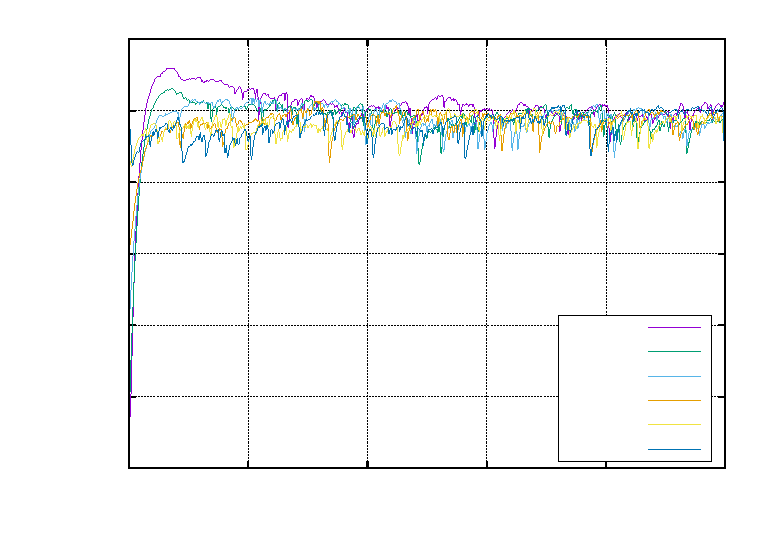
\includegraphics[width={360.00bp},height={252.00bp}]{./Taux_ft_fn}}%
    \gplfronttext
  \end{picture}%
\endgroup
}\label{fig:palier_a}}
    \subfloat[Indice des vides]{\scalebox{0.33}{\small % GNUPLOT: LaTeX picture with Postscript
\begingroup
  \makeatletter
  \providecommand\color[2][]{%
    \GenericError{(gnuplot) \space\space\space\@spaces}{%
      Package color not loaded in conjunction with
      terminal option `colourtext'%
    }{See the gnuplot documentation for explanation.%
    }{Either use 'blacktext' in gnuplot or load the package
      color.sty in LaTeX.}%
    \renewcommand\color[2][]{}%
  }%
  \providecommand\includegraphics[2][]{%
    \GenericError{(gnuplot) \space\space\space\@spaces}{%
      Package graphicx or graphics not loaded%
    }{See the gnuplot documentation for explanation.%
    }{The gnuplot epslatex terminal needs graphicx.sty or graphics.sty.}%
    \renewcommand\includegraphics[2][]{}%
  }%
  \providecommand\rotatebox[2]{#2}%
  \@ifundefined{ifGPcolor}{%
    \newif\ifGPcolor
    \GPcolortrue
  }{}%
  \@ifundefined{ifGPblacktext}{%
    \newif\ifGPblacktext
    \GPblacktextfalse
  }{}%
  % define a \g@addto@macro without @ in the name:
  \let\gplgaddtomacro\g@addto@macro
  % define empty templates for all commands taking text:
  \gdef\gplbacktext{}%
  \gdef\gplfronttext{}%
  \makeatother
  \ifGPblacktext
    % no textcolor at all
    \def\colorrgb#1{}%
    \def\colorgray#1{}%
  \else
    % gray or color?
    \ifGPcolor
      \def\colorrgb#1{\color[rgb]{#1}}%
      \def\colorgray#1{\color[gray]{#1}}%
      \expandafter\def\csname LTw\endcsname{\color{white}}%
      \expandafter\def\csname LTb\endcsname{\color{black}}%
      \expandafter\def\csname LTa\endcsname{\color{black}}%
      \expandafter\def\csname LT0\endcsname{\color[rgb]{1,0,0}}%
      \expandafter\def\csname LT1\endcsname{\color[rgb]{0,1,0}}%
      \expandafter\def\csname LT2\endcsname{\color[rgb]{0,0,1}}%
      \expandafter\def\csname LT3\endcsname{\color[rgb]{1,0,1}}%
      \expandafter\def\csname LT4\endcsname{\color[rgb]{0,1,1}}%
      \expandafter\def\csname LT5\endcsname{\color[rgb]{1,1,0}}%
      \expandafter\def\csname LT6\endcsname{\color[rgb]{0,0,0}}%
      \expandafter\def\csname LT7\endcsname{\color[rgb]{1,0.3,0}}%
      \expandafter\def\csname LT8\endcsname{\color[rgb]{0.5,0.5,0.5}}%
    \else
      % gray
      \def\colorrgb#1{\color{black}}%
      \def\colorgray#1{\color[gray]{#1}}%
      \expandafter\def\csname LTw\endcsname{\color{white}}%
      \expandafter\def\csname LTb\endcsname{\color{black}}%
      \expandafter\def\csname LTa\endcsname{\color{black}}%
      \expandafter\def\csname LT0\endcsname{\color{black}}%
      \expandafter\def\csname LT1\endcsname{\color{black}}%
      \expandafter\def\csname LT2\endcsname{\color{black}}%
      \expandafter\def\csname LT3\endcsname{\color{black}}%
      \expandafter\def\csname LT4\endcsname{\color{black}}%
      \expandafter\def\csname LT5\endcsname{\color{black}}%
      \expandafter\def\csname LT6\endcsname{\color{black}}%
      \expandafter\def\csname LT7\endcsname{\color{black}}%
      \expandafter\def\csname LT8\endcsname{\color{black}}%
    \fi
  \fi
    \setlength{\unitlength}{0.0500bp}%
    \ifx\gptboxheight\undefined%
      \newlength{\gptboxheight}%
      \newlength{\gptboxwidth}%
      \newsavebox{\gptboxtext}%
    \fi%
    \setlength{\fboxrule}{0.5pt}%
    \setlength{\fboxsep}{1pt}%
    \definecolor{tbcol}{rgb}{1,1,1}%
\begin{picture}(7200.00,5040.00)%
    \gplgaddtomacro\gplbacktext{%
      \csname LTb\endcsname%%
      \put(946,1834){\makebox(0,0)[r]{\strut{}$0.62$}}%
      \csname LTb\endcsname%%
      \put(946,2293){\makebox(0,0)[r]{\strut{}$0.64$}}%
      \csname LTb\endcsname%%
      \put(946,2752){\makebox(0,0)[r]{\strut{}$0.66$}}%
      \csname LTb\endcsname%%
      \put(946,3212){\makebox(0,0)[r]{\strut{}$0.68$}}%
      \csname LTb\endcsname%%
      \put(946,3671){\makebox(0,0)[r]{\strut{}$0.7$}}%
      \csname LTb\endcsname%%
      \put(946,4130){\makebox(0,0)[r]{\strut{}$0.72$}}%
      \csname LTb\endcsname%%
      \put(946,4589){\makebox(0,0)[r]{\strut{}$0.74$}}%
      \csname LTb\endcsname%%
      \put(1078,1384){\makebox(0,0){\strut{}$0$}}%
      \csname LTb\endcsname%%
      \put(2223,1384){\makebox(0,0){\strut{}$20$}}%
      \csname LTb\endcsname%%
      \put(3368,1384){\makebox(0,0){\strut{}$40$}}%
      \csname LTb\endcsname%%
      \put(4513,1384){\makebox(0,0){\strut{}$60$}}%
      \csname LTb\endcsname%%
      \put(5658,1384){\makebox(0,0){\strut{}$80$}}%
      \csname LTb\endcsname%%
      \put(6803,1384){\makebox(0,0){\strut{}$100$}}%
    }%
    \gplgaddtomacro\gplfronttext{%
      \csname LTb\endcsname%%
      \put(209,3211){\rotatebox{-270}{\makebox(0,0){\strut{}e}}}%
      \put(3940,1054){\makebox(0,0){\strut{}$\varepsilon_{yy}$ (\%)}}%
      \csname LTb\endcsname%%
      \put(2046,813){\makebox(0,0)[r]{\strut{}$I = 1 \times 10^{-4}$}}%
      \csname LTb\endcsname%%
      \put(2046,513){\makebox(0,0)[r]{\strut{}$I = 1 \times 10^{-3}$}}%
      \csname LTb\endcsname%%
      \put(2046,213){\makebox(0,0)[r]{\strut{}$I = 2 \times 10^{-3}$}}%
      \csname LTb\endcsname%%
      \put(4269,813){\makebox(0,0)[r]{\strut{}$I = 4 \times 10^{-3}$}}%
      \csname LTb\endcsname%%
      \put(4269,513){\makebox(0,0)[r]{\strut{}$I = 6 \times 10^{-3}$}}%
      \csname LTb\endcsname%%
      \put(4269,213){\makebox(0,0)[r]{\strut{}$I = 8 \times 10^{-3}$}}%
      \csname LTb\endcsname%%
      \put(6492,813){\makebox(0,0)[r]{\strut{}$I = 1 \times 10^{-2}$}}%
    }%
    \gplbacktext
    \put(0,0){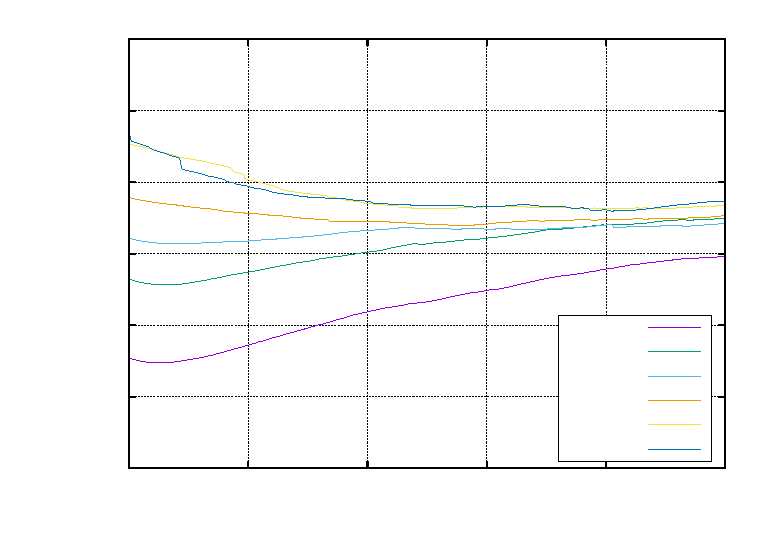
\includegraphics[width={360.00bp},height={252.00bp}]{./RapportVides}}%
    \gplfronttext
  \end{picture}%
\endgroup
}\label{fig:palier_b}}
    \subfloat[Nombre de contacts]{\scalebox{0.33}{\small % GNUPLOT: LaTeX picture with Postscript
\begingroup
  \makeatletter
  \providecommand\color[2][]{%
    \GenericError{(gnuplot) \space\space\space\@spaces}{%
      Package color not loaded in conjunction with
      terminal option `colourtext'%
    }{See the gnuplot documentation for explanation.%
    }{Either use 'blacktext' in gnuplot or load the package
      color.sty in LaTeX.}%
    \renewcommand\color[2][]{}%
  }%
  \providecommand\includegraphics[2][]{%
    \GenericError{(gnuplot) \space\space\space\@spaces}{%
      Package graphicx or graphics not loaded%
    }{See the gnuplot documentation for explanation.%
    }{The gnuplot epslatex terminal needs graphicx.sty or graphics.sty.}%
    \renewcommand\includegraphics[2][]{}%
  }%
  \providecommand\rotatebox[2]{#2}%
  \@ifundefined{ifGPcolor}{%
    \newif\ifGPcolor
    \GPcolortrue
  }{}%
  \@ifundefined{ifGPblacktext}{%
    \newif\ifGPblacktext
    \GPblacktexttrue
  }{}%
  % define a \g@addto@macro without @ in the name:
  \let\gplgaddtomacro\g@addto@macro
  % define empty templates for all commands taking text:
  \gdef\gplbacktext{}%
  \gdef\gplfronttext{}%
  \makeatother
  \ifGPblacktext
    % no textcolor at all
    \def\colorrgb#1{}%
    \def\colorgray#1{}%
  \else
    % gray or color?
    \ifGPcolor
      \def\colorrgb#1{\color[rgb]{#1}}%
      \def\colorgray#1{\color[gray]{#1}}%
      \expandafter\def\csname LTw\endcsname{\color{white}}%
      \expandafter\def\csname LTb\endcsname{\color{black}}%
      \expandafter\def\csname LTa\endcsname{\color{black}}%
      \expandafter\def\csname LT0\endcsname{\color[rgb]{1,0,0}}%
      \expandafter\def\csname LT1\endcsname{\color[rgb]{0,1,0}}%
      \expandafter\def\csname LT2\endcsname{\color[rgb]{0,0,1}}%
      \expandafter\def\csname LT3\endcsname{\color[rgb]{1,0,1}}%
      \expandafter\def\csname LT4\endcsname{\color[rgb]{0,1,1}}%
      \expandafter\def\csname LT5\endcsname{\color[rgb]{1,1,0}}%
      \expandafter\def\csname LT6\endcsname{\color[rgb]{0,0,0}}%
      \expandafter\def\csname LT7\endcsname{\color[rgb]{1,0.3,0}}%
      \expandafter\def\csname LT8\endcsname{\color[rgb]{0.5,0.5,0.5}}%
    \else
      % gray
      \def\colorrgb#1{\color{black}}%
      \def\colorgray#1{\color[gray]{#1}}%
      \expandafter\def\csname LTw\endcsname{\color{white}}%
      \expandafter\def\csname LTb\endcsname{\color{black}}%
      \expandafter\def\csname LTa\endcsname{\color{black}}%
      \expandafter\def\csname LT0\endcsname{\color{black}}%
      \expandafter\def\csname LT1\endcsname{\color{black}}%
      \expandafter\def\csname LT2\endcsname{\color{black}}%
      \expandafter\def\csname LT3\endcsname{\color{black}}%
      \expandafter\def\csname LT4\endcsname{\color{black}}%
      \expandafter\def\csname LT5\endcsname{\color{black}}%
      \expandafter\def\csname LT6\endcsname{\color{black}}%
      \expandafter\def\csname LT7\endcsname{\color{black}}%
      \expandafter\def\csname LT8\endcsname{\color{black}}%
    \fi
  \fi
    \setlength{\unitlength}{0.0500bp}%
    \ifx\gptboxheight\undefined%
      \newlength{\gptboxheight}%
      \newlength{\gptboxwidth}%
      \newsavebox{\gptboxtext}%
    \fi%
    \setlength{\fboxrule}{0.5pt}%
    \setlength{\fboxsep}{1pt}%
    \definecolor{tbcol}{rgb}{1,1,1}%
\begin{picture}(7200.00,5040.00)%
    \gplgaddtomacro\gplbacktext{%
      \csname LTb\endcsname%%
      \put(814,704){\makebox(0,0)[r]{\strut{}$2$}}%
      \csname LTb\endcsname%%
      \put(814,1527){\makebox(0,0)[r]{\strut{}$2.2$}}%
      \csname LTb\endcsname%%
      \put(814,2350){\makebox(0,0)[r]{\strut{}$2.4$}}%
      \csname LTb\endcsname%%
      \put(814,3173){\makebox(0,0)[r]{\strut{}$2.6$}}%
      \csname LTb\endcsname%%
      \put(814,3996){\makebox(0,0)[r]{\strut{}$2.8$}}%
      \csname LTb\endcsname%%
      \put(814,4819){\makebox(0,0)[r]{\strut{}$3$}}%
      \csname LTb\endcsname%%
      \put(946,484){\makebox(0,0){\strut{}$0$}}%
      \csname LTb\endcsname%%
      \put(2117,484){\makebox(0,0){\strut{}$2$}}%
      \csname LTb\endcsname%%
      \put(3289,484){\makebox(0,0){\strut{}$4$}}%
      \csname LTb\endcsname%%
      \put(4460,484){\makebox(0,0){\strut{}$6$}}%
      \csname LTb\endcsname%%
      \put(5632,484){\makebox(0,0){\strut{}$8$}}%
      \csname LTb\endcsname%%
      \put(6803,484){\makebox(0,0){\strut{}$10$}}%
    }%
    \gplgaddtomacro\gplfronttext{%
      \csname LTb\endcsname%%
      \put(209,2761){\rotatebox{-270}{\makebox(0,0){\strut{}$N_{contacts}/N_{particules}$}}}%
      \put(3874,154){\makebox(0,0){\strut{}$\varepsilon_{yy}$ (\%)}}%
      \csname LTb\endcsname%%
      \put(5960,4639){\makebox(0,0)[r]{\strut{}$\mu = 0$}}%
      \csname LTb\endcsname%%
      \put(5960,4405){\makebox(0,0)[r]{\strut{}$\mu = 0.1$}}%
      \csname LTb\endcsname%%
      \put(5960,4171){\makebox(0,0)[r]{\strut{}$\mu = 0.2$}}%
      \csname LTb\endcsname%%
      \put(5960,3937){\makebox(0,0)[r]{\strut{}$\mu = 0.3$}}%
      \csname LTb\endcsname%%
      \put(5960,3703){\makebox(0,0)[r]{\strut{}$\mu = 0.4$}}%
      \csname LTb\endcsname%%
      \put(5960,3469){\makebox(0,0)[r]{\strut{}$\mu = 0.5$}}%
    }%
    \gplbacktext
    \put(0,0){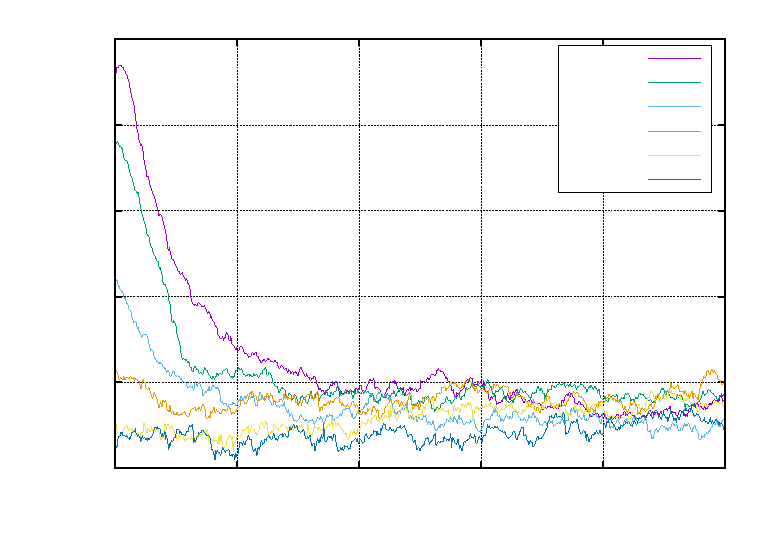
\includegraphics[width={360.00bp},height={252.00bp}]{./NombreContacts}}%
    \gplfronttext
  \end{picture}%
\endgroup
}\label{fig:palier_c}}
    \caption{Tendance des grandeurs à l’état critique}
    \label{fig:Palier}
\end{figure}

Grâce aux courbes de contraintes (\autoref{fig:comparaison}), le comportement différencié des échantillons est désormais visible.  
On observe que, pour différentes valeurs de $\mu$ en compression isotrope, on obtient des échantillons avec différentes compacités, ce qui conduit à des comportements très distincts.  

Selon la \autoref{fig:Palier}, lorsque la déformation dépasse environ 8~\%, les courbes de la norme des forces, de l’indice des vides et du nombre de contacts (ou nombre de coordination) tendent progressivement vers un même palier.  
Concernant la contrainte, le pic augmente avec la compacité du volume élémentaire (VE). Un VE très lâche ne présente pas de pic. Pour de grandes déformations, tous les échantillons tendent vers un même palier, appelé état critique.  

Ces simulations confirment ainsi la théorie de l’état critique en mécanique des sols : une fois cet état atteint, la déformation plastique peut croître indéfiniment à contrainte et indice des vides constants.  
Cet état est celui utilisé pour la modélisation des écoulements.

\subsubsection{Cercle de Mohr}

\begin{figure}[h!]
    \centering
    \begin{subfigure}[b]{0.48\textwidth}
        \centering
        \scalebox{0.6}{\small % GNUPLOT: LaTeX picture with Postscript
\begingroup
  \makeatletter
  \providecommand\color[2][]{%
    \GenericError{(gnuplot) \space\space\space\@spaces}{%
      Package color not loaded in conjunction with
      terminal option `colourtext'%
    }{See the gnuplot documentation for explanation.%
    }{Either use 'blacktext' in gnuplot or load the package
      color.sty in LaTeX.}%
    \renewcommand\color[2][]{}%
  }%
  \providecommand\includegraphics[2][]{%
    \GenericError{(gnuplot) \space\space\space\@spaces}{%
      Package graphicx or graphics not loaded%
    }{See the gnuplot documentation for explanation.%
    }{The gnuplot epslatex terminal needs graphicx.sty or graphics.sty.}%
    \renewcommand\includegraphics[2][]{}%
  }%
  \providecommand\rotatebox[2]{#2}%
  \@ifundefined{ifGPcolor}{%
    \newif\ifGPcolor
    \GPcolortrue
  }{}%
  \@ifundefined{ifGPblacktext}{%
    \newif\ifGPblacktext
    \GPblacktextfalse
  }{}%
  % define a \g@addto@macro without @ in the name:
  \let\gplgaddtomacro\g@addto@macro
  % define empty templates for all commands taking text:
  \gdef\gplbacktext{}%
  \gdef\gplfronttext{}%
  \makeatother
  \ifGPblacktext
    % no textcolor at all
    \def\colorrgb#1{}%
    \def\colorgray#1{}%
  \else
    % gray or color?
    \ifGPcolor
      \def\colorrgb#1{\color[rgb]{#1}}%
      \def\colorgray#1{\color[gray]{#1}}%
      \expandafter\def\csname LTw\endcsname{\color{white}}%
      \expandafter\def\csname LTb\endcsname{\color{black}}%
      \expandafter\def\csname LTa\endcsname{\color{black}}%
      \expandafter\def\csname LT0\endcsname{\color[rgb]{1,0,0}}%
      \expandafter\def\csname LT1\endcsname{\color[rgb]{0,1,0}}%
      \expandafter\def\csname LT2\endcsname{\color[rgb]{0,0,1}}%
      \expandafter\def\csname LT3\endcsname{\color[rgb]{1,0,1}}%
      \expandafter\def\csname LT4\endcsname{\color[rgb]{0,1,1}}%
      \expandafter\def\csname LT5\endcsname{\color[rgb]{1,1,0}}%
      \expandafter\def\csname LT6\endcsname{\color[rgb]{0,0,0}}%
      \expandafter\def\csname LT7\endcsname{\color[rgb]{1,0.3,0}}%
      \expandafter\def\csname LT8\endcsname{\color[rgb]{0.5,0.5,0.5}}%
    \else
      % gray
      \def\colorrgb#1{\color{black}}%
      \def\colorgray#1{\color[gray]{#1}}%
      \expandafter\def\csname LTw\endcsname{\color{white}}%
      \expandafter\def\csname LTb\endcsname{\color{black}}%
      \expandafter\def\csname LTa\endcsname{\color{black}}%
      \expandafter\def\csname LT0\endcsname{\color{black}}%
      \expandafter\def\csname LT1\endcsname{\color{black}}%
      \expandafter\def\csname LT2\endcsname{\color{black}}%
      \expandafter\def\csname LT3\endcsname{\color{black}}%
      \expandafter\def\csname LT4\endcsname{\color{black}}%
      \expandafter\def\csname LT5\endcsname{\color{black}}%
      \expandafter\def\csname LT6\endcsname{\color{black}}%
      \expandafter\def\csname LT7\endcsname{\color{black}}%
      \expandafter\def\csname LT8\endcsname{\color{black}}%
    \fi
  \fi
    \setlength{\unitlength}{0.0500bp}%
    \ifx\gptboxheight\undefined%
      \newlength{\gptboxheight}%
      \newlength{\gptboxwidth}%
      \newsavebox{\gptboxtext}%
    \fi%
    \setlength{\fboxrule}{0.5pt}%
    \setlength{\fboxsep}{1pt}%
    \definecolor{tbcol}{rgb}{1,1,1}%
\begin{picture}(7200.00,5040.00)%
    \gplgaddtomacro\gplbacktext{%
      \csname LTb\endcsname%%
      \put(814,1785){\makebox(0,0)[r]{\strut{}$0$}}%
      \put(814,2273){\makebox(0,0)[r]{\strut{}$50$}}%
      \put(814,2762){\makebox(0,0)[r]{\strut{}$100$}}%
      \put(814,3250){\makebox(0,0)[r]{\strut{}$150$}}%
      \put(814,3738){\makebox(0,0)[r]{\strut{}$200$}}%
      \put(946,1565){\makebox(0,0){\strut{}$0$}}%
      \put(1922,1565){\makebox(0,0){\strut{}$100$}}%
      \put(2898,1565){\makebox(0,0){\strut{}$200$}}%
      \put(3875,1565){\makebox(0,0){\strut{}$300$}}%
      \put(4851,1565){\makebox(0,0){\strut{}$400$}}%
      \put(5827,1565){\makebox(0,0){\strut{}$500$}}%
      \put(6803,1565){\makebox(0,0){\strut{}$600$}}%
      \colorrgb{0.00,0.00,1.00}%%
      \put(6369,3409){\makebox(0,0)[l]{\strut{}$\varphi_1 = 17.36^\circ$}}%
      \colorrgb{1.00,0.00,0.00}%%
      \put(5149,3067){\makebox(0,0)[l]{\strut{}$\varphi_2 = \varphi_3 = 17.92^\circ$}}%
      \colorrgb{0.00,0.00,0.00}%%
      \put(3875,2957){\makebox(0,0){\strut{}\rotatebox{17}{$\tau= \sigma_n \times \tan(\varphi) + c$}}}%
    }%
    \gplgaddtomacro\gplfronttext{%
      \csname LTb\endcsname%%
      \put(209,2761){\rotatebox{-270}{\makebox(0,0){\strut{}$\tau$ (kPa)}}}%
      \put(3874,1235){\makebox(0,0){\strut{}$\sigma_n$ (kPa)}}%
    }%
    \gplbacktext
    \put(0,0){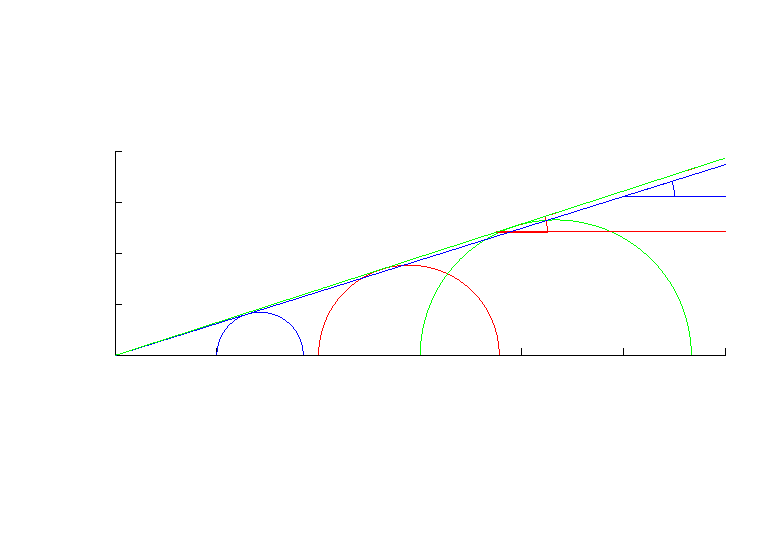
\includegraphics[width={360.00bp},height={252.00bp}]{CercleMohr}}%
    \gplfronttext
  \end{picture}%
\endgroup
}
        \caption{Dense}
        \label{fig:cercle_dense}
    \end{subfigure}
    \hfill
    \begin{subfigure}[b]{0.48\textwidth}
        \centering
        \scalebox{0.65}{\small % GNUPLOT: LaTeX picture with Postscript
\begingroup
  \makeatletter
  \providecommand\color[2][]{%
    \GenericError{(gnuplot) \space\space\space\@spaces}{%
      Package color not loaded in conjunction with
      terminal option `colourtext'%
    }{See the gnuplot documentation for explanation.%
    }{Either use 'blacktext' in gnuplot or load the package
      color.sty in LaTeX.}%
    \renewcommand\color[2][]{}%
  }%
  \providecommand\includegraphics[2][]{%
    \GenericError{(gnuplot) \space\space\space\@spaces}{%
      Package graphicx or graphics not loaded%
    }{See the gnuplot documentation for explanation.%
    }{The gnuplot epslatex terminal needs graphicx.sty or graphics.sty.}%
    \renewcommand\includegraphics[2][]{}%
  }%
  \providecommand\rotatebox[2]{#2}%
  \@ifundefined{ifGPcolor}{%
    \newif\ifGPcolor
    \GPcolortrue
  }{}%
  \@ifundefined{ifGPblacktext}{%
    \newif\ifGPblacktext
    \GPblacktextfalse
  }{}%
  % define a \g@addto@macro without @ in the name:
  \let\gplgaddtomacro\g@addto@macro
  % define empty templates for all commands taking text:
  \gdef\gplbacktext{}%
  \gdef\gplfronttext{}%
  \makeatother
  \ifGPblacktext
    % no textcolor at all
    \def\colorrgb#1{}%
    \def\colorgray#1{}%
  \else
    % gray or color?
    \ifGPcolor
      \def\colorrgb#1{\color[rgb]{#1}}%
      \def\colorgray#1{\color[gray]{#1}}%
      \expandafter\def\csname LTw\endcsname{\color{white}}%
      \expandafter\def\csname LTb\endcsname{\color{black}}%
      \expandafter\def\csname LTa\endcsname{\color{black}}%
      \expandafter\def\csname LT0\endcsname{\color[rgb]{1,0,0}}%
      \expandafter\def\csname LT1\endcsname{\color[rgb]{0,1,0}}%
      \expandafter\def\csname LT2\endcsname{\color[rgb]{0,0,1}}%
      \expandafter\def\csname LT3\endcsname{\color[rgb]{1,0,1}}%
      \expandafter\def\csname LT4\endcsname{\color[rgb]{0,1,1}}%
      \expandafter\def\csname LT5\endcsname{\color[rgb]{1,1,0}}%
      \expandafter\def\csname LT6\endcsname{\color[rgb]{0,0,0}}%
      \expandafter\def\csname LT7\endcsname{\color[rgb]{1,0.3,0}}%
      \expandafter\def\csname LT8\endcsname{\color[rgb]{0.5,0.5,0.5}}%
    \else
      % gray
      \def\colorrgb#1{\color{black}}%
      \def\colorgray#1{\color[gray]{#1}}%
      \expandafter\def\csname LTw\endcsname{\color{white}}%
      \expandafter\def\csname LTb\endcsname{\color{black}}%
      \expandafter\def\csname LTa\endcsname{\color{black}}%
      \expandafter\def\csname LT0\endcsname{\color{black}}%
      \expandafter\def\csname LT1\endcsname{\color{black}}%
      \expandafter\def\csname LT2\endcsname{\color{black}}%
      \expandafter\def\csname LT3\endcsname{\color{black}}%
      \expandafter\def\csname LT4\endcsname{\color{black}}%
      \expandafter\def\csname LT5\endcsname{\color{black}}%
      \expandafter\def\csname LT6\endcsname{\color{black}}%
      \expandafter\def\csname LT7\endcsname{\color{black}}%
      \expandafter\def\csname LT8\endcsname{\color{black}}%
    \fi
  \fi
    \setlength{\unitlength}{0.0500bp}%
    \ifx\gptboxheight\undefined%
      \newlength{\gptboxheight}%
      \newlength{\gptboxwidth}%
      \newsavebox{\gptboxtext}%
    \fi%
    \setlength{\fboxrule}{0.5pt}%
    \setlength{\fboxsep}{1pt}%
    \definecolor{tbcol}{rgb}{1,1,1}%
\begin{picture}(7200.00,5040.00)%
    \gplgaddtomacro\gplbacktext{%
      \csname LTb\endcsname%%
      \put(814,1942){\makebox(0,0)[r]{\strut{}$0$}}%
      \put(814,2176){\makebox(0,0)[r]{\strut{}$20$}}%
      \put(814,2410){\makebox(0,0)[r]{\strut{}$40$}}%
      \put(814,2644){\makebox(0,0)[r]{\strut{}$60$}}%
      \put(814,2879){\makebox(0,0)[r]{\strut{}$80$}}%
      \put(814,3113){\makebox(0,0)[r]{\strut{}$100$}}%
      \put(814,3347){\makebox(0,0)[r]{\strut{}$120$}}%
      \put(814,3581){\makebox(0,0)[r]{\strut{}$140$}}%
      \put(946,1722){\makebox(0,0){\strut{}$0$}}%
      \put(2117,1722){\makebox(0,0){\strut{}$100$}}%
      \put(3289,1722){\makebox(0,0){\strut{}$200$}}%
      \put(4460,1722){\makebox(0,0){\strut{}$300$}}%
      \put(5632,1722){\makebox(0,0){\strut{}$400$}}%
      \put(6803,1722){\makebox(0,0){\strut{}$500$}}%
      \colorrgb{0.00,0.00,1.00}%%
      \put(1649,2058){\makebox(0,0)[l]{\strut{}$\varphi_1 = 9.49^\circ$}}%
      \colorrgb{1.00,0.00,0.00}%%
      \put(3052,2130){\makebox(0,0)[l]{\strut{}$\varphi_2 = 10.24^\circ$}}%
      \colorrgb{0.00,1.00,0.00}%%
      \put(4498,2318){\makebox(0,0)[l]{\strut{}$\varphi_3 = 12.13^\circ$}}%
      \colorrgb{0.00,0.00,0.00}%%
      \put(3875,2843){\makebox(0,0){\strut{}\rotatebox{12}{$\tau= \sigma_n \times \tan(\varphi) + c$}}}%
    }%
    \gplgaddtomacro\gplfronttext{%
      \csname LTb\endcsname%%
      \put(209,2761){\rotatebox{-270}{\makebox(0,0){\strut{}$\tau$ (kPa)}}}%
      \put(3874,1392){\makebox(0,0){\strut{}$\sigma_n$ (kPa)}}%
    }%
    \gplbacktext
    \put(0,0){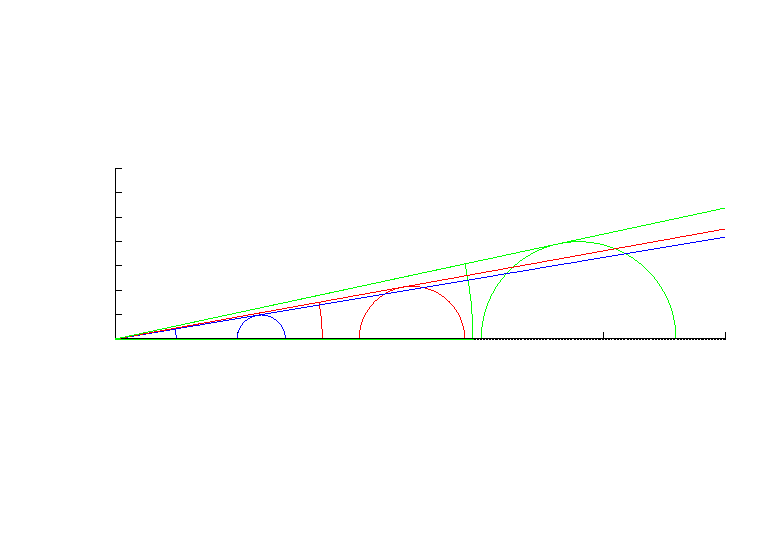
\includegraphics[width={360.00bp},height={252.00bp}]{LACHE_CercleMohr}}%
    \gplfronttext
  \end{picture}%
\endgroup
}
        \caption{Lâche}
        \label{fig:cercle_lache}
    \end{subfigure}
    \caption{Cercles de Mohr: les cercles bleu, rouge et vert représentent respectivement $\sigma_3 = 100, 200, 300$ kPa}
    \label{fig:CercleDuMohr}
\end{figure}

Un point particulier de la méthode DEM est que l’on agit uniquement sur les paramètres microscopiques, alors que les comportements à grande échelle émergent naturellement.  
Cette propriété peut être vérifiée en comparant avec les comportements macroscopiques bien connus en mécanique des sols.  

Le cercle de Mohr est une méthode bien connue pour identifier la résistance au cisaillement maximale du sol.  
À partir de ses courbes, on peut déterminer la cohésion $c$ et l’angle de frottement interne $\varphi$ selon la relation :
\begin{equation}
    \tau = \sigma_n \tan(\varphi) + c
    \label{eq:tangentMohr}
\end{equation}

Le point quadrature gauche de chaque cercle sur la \autoref{fig:CercleDuMohr} correspond à la contrainte $\sigma_3$, tandis que le point droit représente la contrainte à l’état considéré.  

Lors d’essais triaxiaux réalisés sur un même échantillon avec différentes valeurs de $\sigma_3$, plusieurs cercles peuvent être tracés. La droite tangente à ces cercles est la droite limite de Mohr-Coulomb, de la forme \eqref{eq:tangentMohr}.  

Nous nous intéressons ici à deux états importants : le pic et l’état critique.  
Pour un échantillon donné, le pic correspond à la contrainte maximale avant rupture par cisaillement.  
La pente de la droite tangente aux cercles, soit $\tan(\varphi) = \mu$, reflète le frottement interne à l’état considéré.  

La \autoref{fig:CercleDuMohr} donne la valeur de $\mu_{\text{transitoire}}$ au pic, c’est-à-dire lorsque la résistance au cisaillement due aux contacts frottants entre grains est maximale.  
Naturellement, un sol dense (figure \ref{fig:cercle_dense}) présente un angle de frottement $\varphi$ plus élevé qu’un sol lâche (figure \ref{fig:cercle_lache}).  

Le $\mu_{\text{résiduel}}$ correspond à la pente de la droite tangente au cercle de Mohr à l’état critique.  
On considère généralement que ce $\mu_{\text{résiduel}}$ est une valeur stationnaire.  

Ce paramètre est essentiel pour intégrer le modèle MPMxDEM, car le sol en écoulement se comporte comme un matériau à l’état critique :  
il subit des déformations très importantes, la structure initiale est totalement détruite, et la résistance interne ne dépend plus que du frottement résiduel entre grains.  

Dans notre cas, le matériau étudié est du sable sec. Le point d’intersection entre la droite tangente aux cercles et l’axe vertical, selon la théorie, doit être nul, ce qui correspond à une cohésion nulle ($c=0$).

\subsection{Recherche sur l'impact dynamique}
\begin{table}[h!]
\centering
\begin{tabular}{|c|c|c|}
\hline
$ I < 10^{-3} $ & $ 10^{-3} < I < 10^{-1} $ & $ I > 10^{-1} $ \\ 
\hline
Solides & Fluides & Gaz \\  
\hline
\end{tabular}
\caption{Nombre d’inertie}
\label{tab:nombreInertie}
\end{table}

Dans cette section, nous étudions le nombre d’inertie, qui est un verrou mentionné dans l’objet de la thèse.  
L’augmentation du nombre d’inertie dans un essai triaxial correspond à une augmentation de la vitesse imposée.  
Normalement, la valeur recommandée de $I$ pour les expériences DEM dans le cadre expérimental est $I < 10^{-7}$.  
Cependant, en simulation, cette valeur est pratiquement inatteignable en raison du coût temporel élevé.  
Ainsi, le tableau \ref{tab:nombreInertie} présente les valeurs recommandées par le comité de modélisation des sols.  
Lors de la réalisation d’un essai triaxial numérique, pour atteindre un état quasi-statique, on choisit généralement $I < 10^{-3}$.  
À ce stade, le tenseur des contraintes est symétrique et les composantes $\sigma_{xx}$ ou $\sigma_{zz}$ sont approximativement stables et proches de la contrainte de confinement imposée.  
Cependant, dans l’objectif de modéliser un écoulement, nous nous intéressons à des valeurs de $I$ plus élevées, comprises entre $10^{-3}$ et $10^{-1}$, afin d’obtenir un comportement fluide.

\begin{figure}[h!]
\centering \small
\scalebox{0.5}{% GNUPLOT: LaTeX picture with Postscript
\begingroup
  \makeatletter
  \providecommand\color[2][]{%
    \GenericError{(gnuplot) \space\space\space\@spaces}{%
      Package color not loaded in conjunction with
      terminal option `colourtext'%
    }{See the gnuplot documentation for explanation.%
    }{Either use 'blacktext' in gnuplot or load the package
      color.sty in LaTeX.}%
    \renewcommand\color[2][]{}%
  }%
  \providecommand\includegraphics[2][]{%
    \GenericError{(gnuplot) \space\space\space\@spaces}{%
      Package graphicx or graphics not loaded%
    }{See the gnuplot documentation for explanation.%
    }{The gnuplot epslatex terminal needs graphicx.sty or graphics.sty.}%
    \renewcommand\includegraphics[2][]{}%
  }%
  \providecommand\rotatebox[2]{#2}%
  \@ifundefined{ifGPcolor}{%
    \newif\ifGPcolor
    \GPcolortrue
  }{}%
  \@ifundefined{ifGPblacktext}{%
    \newif\ifGPblacktext
    \GPblacktextfalse
  }{}%
  % define a \g@addto@macro without @ in the name:
  \let\gplgaddtomacro\g@addto@macro
  % define empty templates for all commands taking text:
  \gdef\gplbacktext{}%
  \gdef\gplfronttext{}%
  \makeatother
  \ifGPblacktext
    % no textcolor at all
    \def\colorrgb#1{}%
    \def\colorgray#1{}%
  \else
    % gray or color?
    \ifGPcolor
      \def\colorrgb#1{\color[rgb]{#1}}%
      \def\colorgray#1{\color[gray]{#1}}%
      \expandafter\def\csname LTw\endcsname{\color{white}}%
      \expandafter\def\csname LTb\endcsname{\color{black}}%
      \expandafter\def\csname LTa\endcsname{\color{black}}%
      \expandafter\def\csname LT0\endcsname{\color[rgb]{1,0,0}}%
      \expandafter\def\csname LT1\endcsname{\color[rgb]{0,1,0}}%
      \expandafter\def\csname LT2\endcsname{\color[rgb]{0,0,1}}%
      \expandafter\def\csname LT3\endcsname{\color[rgb]{1,0,1}}%
      \expandafter\def\csname LT4\endcsname{\color[rgb]{0,1,1}}%
      \expandafter\def\csname LT5\endcsname{\color[rgb]{1,1,0}}%
      \expandafter\def\csname LT6\endcsname{\color[rgb]{0,0,0}}%
      \expandafter\def\csname LT7\endcsname{\color[rgb]{1,0.3,0}}%
      \expandafter\def\csname LT8\endcsname{\color[rgb]{0.5,0.5,0.5}}%
    \else
      % gray
      \def\colorrgb#1{\color{black}}%
      \def\colorgray#1{\color[gray]{#1}}%
      \expandafter\def\csname LTw\endcsname{\color{white}}%
      \expandafter\def\csname LTb\endcsname{\color{black}}%
      \expandafter\def\csname LTa\endcsname{\color{black}}%
      \expandafter\def\csname LT0\endcsname{\color{black}}%
      \expandafter\def\csname LT1\endcsname{\color{black}}%
      \expandafter\def\csname LT2\endcsname{\color{black}}%
      \expandafter\def\csname LT3\endcsname{\color{black}}%
      \expandafter\def\csname LT4\endcsname{\color{black}}%
      \expandafter\def\csname LT5\endcsname{\color{black}}%
      \expandafter\def\csname LT6\endcsname{\color{black}}%
      \expandafter\def\csname LT7\endcsname{\color{black}}%
      \expandafter\def\csname LT8\endcsname{\color{black}}%
    \fi
  \fi
    \setlength{\unitlength}{0.0500bp}%
    \ifx\gptboxheight\undefined%
      \newlength{\gptboxheight}%
      \newlength{\gptboxwidth}%
      \newsavebox{\gptboxtext}%
    \fi%
    \setlength{\fboxrule}{0.5pt}%
    \setlength{\fboxsep}{1pt}%
    \definecolor{tbcol}{rgb}{1,1,1}%
\begin{picture}(7200.00,5040.00)%
    \gplgaddtomacro\gplbacktext{%
      \csname LTb\endcsname%%
      \put(946,1124){\makebox(0,0)[r]{\strut{}$0$}}%
      \csname LTb\endcsname%%
      \put(946,1740){\makebox(0,0)[r]{\strut{}$200$}}%
      \csname LTb\endcsname%%
      \put(946,2356){\makebox(0,0)[r]{\strut{}$400$}}%
      \csname LTb\endcsname%%
      \put(946,2972){\makebox(0,0)[r]{\strut{}$600$}}%
      \csname LTb\endcsname%%
      \put(946,3587){\makebox(0,0)[r]{\strut{}$800$}}%
      \csname LTb\endcsname%%
      \put(946,4203){\makebox(0,0)[r]{\strut{}$1000$}}%
      \csname LTb\endcsname%%
      \put(946,4819){\makebox(0,0)[r]{\strut{}$1200$}}%
      \csname LTb\endcsname%%
      \put(1078,904){\makebox(0,0){\strut{}$0$}}%
      \csname LTb\endcsname%%
      \put(2073,904){\makebox(0,0){\strut{}$5$}}%
      \csname LTb\endcsname%%
      \put(3069,904){\makebox(0,0){\strut{}$10$}}%
      \csname LTb\endcsname%%
      \put(4064,904){\makebox(0,0){\strut{}$15$}}%
      \csname LTb\endcsname%%
      \put(5060,904){\makebox(0,0){\strut{}$20$}}%
      \csname LTb\endcsname%%
      \put(6055,904){\makebox(0,0){\strut{}$25$}}%
      \put(6187,1124){\makebox(0,0)[l]{\strut{}$-1$}}%
      \put(6187,1494){\makebox(0,0)[l]{\strut{}$0$}}%
      \put(6187,1863){\makebox(0,0)[l]{\strut{}$1$}}%
      \put(6187,2233){\makebox(0,0)[l]{\strut{}$2$}}%
      \put(6187,2602){\makebox(0,0)[l]{\strut{}$3$}}%
      \put(6187,2972){\makebox(0,0)[l]{\strut{}$4$}}%
      \put(6187,3341){\makebox(0,0)[l]{\strut{}$5$}}%
      \put(6187,3711){\makebox(0,0)[l]{\strut{}$6$}}%
      \put(6187,4080){\makebox(0,0)[l]{\strut{}$7$}}%
      \put(6187,4450){\makebox(0,0)[l]{\strut{}$8$}}%
      \put(6187,4819){\makebox(0,0)[l]{\strut{}$9$}}%
      \colorrgb{0.58,0.00,0.83}%%
      \put(1304,3100){\makebox(0,0)[l]{\strut{}631.86}}%
      \colorrgb{0.00,0.62,0.45}%%
      \put(1363,3715){\makebox(0,0)[l]{\strut{}831.59}}%
      \colorrgb{0.34,0.71,0.91}%%
      \put(1423,4379){\makebox(0,0)[l]{\strut{}1047.16}}%
    }%
    \gplgaddtomacro\gplfronttext{%
      \csname LTb\endcsname%%
      \put(341,2971){\rotatebox{-270}{\makebox(0,0){\strut{}q (kPa)}}}%
      \put(6693,2971){\rotatebox{-270}{\makebox(0,0){\strut{}$\varepsilon_v$ (\%)}}}%
      \put(3566,794){\makebox(0,0){\strut{}$\varepsilon_{yy}$ (\%)}}%
      \csname LTb\endcsname%%
      \put(2783,483){\makebox(0,0)[r]{\strut{}$\sigma_3 = 100\ \text{kPa}$}}%
      \csname LTb\endcsname%%
      \put(2783,283){\makebox(0,0)[r]{\strut{}$\sigma_3 = 200\ \text{kPa}$}}%
      \csname LTb\endcsname%%
      \put(5318,483){\makebox(0,0)[r]{\strut{}$\sigma_3 = 300\ \text{kPa}$}}%
    }%
    \gplbacktext
    \put(0,0){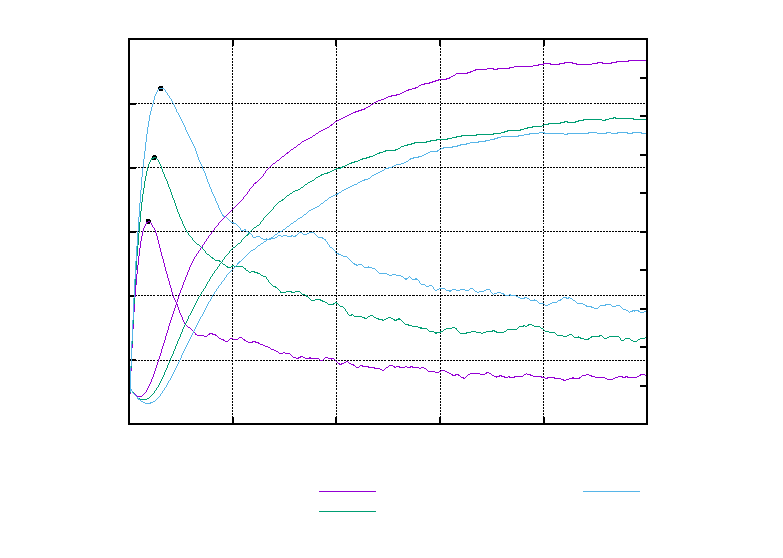
\includegraphics[width={360.00bp},height={252.00bp}]{./10-2}}%
    \gplfronttext
  \end{picture}%
\endgroup
}
\caption{Réponses macroscopiques des essais triaxiaux rapides ($I \approx 10^{-2}$)}
\label{fig:contrainteRapide}
\end{figure}

La figure~\ref{fig:contrainteRapide} montre clairement que plus le nombre d’inertie est élevé, plus le pic de contrainte est marqué et plus la contrainte de confinement présente de fortes fluctuations.  
En utilisant ces valeurs, nous traçons les cercles de Mohr comme suit :

\begin{figure}[htbp]
    \centering \small
    \begin{subfigure}[b]{0.49\textwidth}
        \centering \small
        \scalebox{0.5}{% GNUPLOT: LaTeX picture with Postscript
\begingroup
  \makeatletter
  \providecommand\color[2][]{%
    \GenericError{(gnuplot) \space\space\space\@spaces}{%
      Package color not loaded in conjunction with
      terminal option `colourtext'%
    }{See the gnuplot documentation for explanation.%
    }{Either use 'blacktext' in gnuplot or load the package
      color.sty in LaTeX.}%
    \renewcommand\color[2][]{}%
  }%
  \providecommand\includegraphics[2][]{%
    \GenericError{(gnuplot) \space\space\space\@spaces}{%
      Package graphicx or graphics not loaded%
    }{See the gnuplot documentation for explanation.%
    }{The gnuplot epslatex terminal needs graphicx.sty or graphics.sty.}%
    \renewcommand\includegraphics[2][]{}%
  }%
  \providecommand\rotatebox[2]{#2}%
  \@ifundefined{ifGPcolor}{%
    \newif\ifGPcolor
    \GPcolortrue
  }{}%
  \@ifundefined{ifGPblacktext}{%
    \newif\ifGPblacktext
    \GPblacktextfalse
  }{}%
  % define a \g@addto@macro without @ in the name:
  \let\gplgaddtomacro\g@addto@macro
  % define empty templates for all commands taking text:
  \gdef\gplbacktext{}%
  \gdef\gplfronttext{}%
  \makeatother
  \ifGPblacktext
    % no textcolor at all
    \def\colorrgb#1{}%
    \def\colorgray#1{}%
  \else
    % gray or color?
    \ifGPcolor
      \def\colorrgb#1{\color[rgb]{#1}}%
      \def\colorgray#1{\color[gray]{#1}}%
      \expandafter\def\csname LTw\endcsname{\color{white}}%
      \expandafter\def\csname LTb\endcsname{\color{black}}%
      \expandafter\def\csname LTa\endcsname{\color{black}}%
      \expandafter\def\csname LT0\endcsname{\color[rgb]{1,0,0}}%
      \expandafter\def\csname LT1\endcsname{\color[rgb]{0,1,0}}%
      \expandafter\def\csname LT2\endcsname{\color[rgb]{0,0,1}}%
      \expandafter\def\csname LT3\endcsname{\color[rgb]{1,0,1}}%
      \expandafter\def\csname LT4\endcsname{\color[rgb]{0,1,1}}%
      \expandafter\def\csname LT5\endcsname{\color[rgb]{1,1,0}}%
      \expandafter\def\csname LT6\endcsname{\color[rgb]{0,0,0}}%
      \expandafter\def\csname LT7\endcsname{\color[rgb]{1,0.3,0}}%
      \expandafter\def\csname LT8\endcsname{\color[rgb]{0.5,0.5,0.5}}%
    \else
      % gray
      \def\colorrgb#1{\color{black}}%
      \def\colorgray#1{\color[gray]{#1}}%
      \expandafter\def\csname LTw\endcsname{\color{white}}%
      \expandafter\def\csname LTb\endcsname{\color{black}}%
      \expandafter\def\csname LTa\endcsname{\color{black}}%
      \expandafter\def\csname LT0\endcsname{\color{black}}%
      \expandafter\def\csname LT1\endcsname{\color{black}}%
      \expandafter\def\csname LT2\endcsname{\color{black}}%
      \expandafter\def\csname LT3\endcsname{\color{black}}%
      \expandafter\def\csname LT4\endcsname{\color{black}}%
      \expandafter\def\csname LT5\endcsname{\color{black}}%
      \expandafter\def\csname LT6\endcsname{\color{black}}%
      \expandafter\def\csname LT7\endcsname{\color{black}}%
      \expandafter\def\csname LT8\endcsname{\color{black}}%
    \fi
  \fi
    \setlength{\unitlength}{0.0500bp}%
    \ifx\gptboxheight\undefined%
      \newlength{\gptboxheight}%
      \newlength{\gptboxwidth}%
      \newsavebox{\gptboxtext}%
    \fi%
    \setlength{\fboxrule}{0.5pt}%
    \setlength{\fboxsep}{1pt}%
    \definecolor{tbcol}{rgb}{1,1,1}%
\begin{picture}(7200.00,5040.00)%
    \gplgaddtomacro\gplbacktext{%
      \csname LTb\endcsname%%
      \put(814,2125){\makebox(0,0)[r]{\strut{}$0$}}%
      \put(814,2543){\makebox(0,0)[r]{\strut{}$50$}}%
      \put(814,2962){\makebox(0,0)[r]{\strut{}$100$}}%
      \put(814,3380){\makebox(0,0)[r]{\strut{}$150$}}%
      \put(814,3798){\makebox(0,0)[r]{\strut{}$200$}}%
      \put(946,1905){\makebox(0,0){\strut{}$0$}}%
      \put(1783,1905){\makebox(0,0){\strut{}$100$}}%
      \put(2619,1905){\makebox(0,0){\strut{}$200$}}%
      \put(3456,1905){\makebox(0,0){\strut{}$300$}}%
      \put(4293,1905){\makebox(0,0){\strut{}$400$}}%
      \put(5130,1905){\makebox(0,0){\strut{}$500$}}%
      \put(5966,1905){\makebox(0,0){\strut{}$600$}}%
      \put(6803,1905){\makebox(0,0){\strut{}$700$}}%
      \colorrgb{0.90,0.12,0.06}%%
      \put(1448,2224){\makebox(0,0)[l]{\strut{}$\varphi = 24.84^\circ$}}%
      \put(1030,2032){\makebox(0,0)[l]{\strut{}c = -1.12}}%
    }%
    \gplgaddtomacro\gplfronttext{%
      \csname LTb\endcsname%%
      \put(209,2961){\rotatebox{-270}{\makebox(0,0){\strut{}$\tau$ (kPa)}}}%
      \put(3874,1575){\makebox(0,0){\strut{}$\sigma_n$ (kPa)}}%
      \csname LTb\endcsname%%
      \put(3091,363){\makebox(0,0)[r]{\strut{}$\sigma_3 = 100\ \text{kPa}$}}%
      \csname LTb\endcsname%%
      \put(3091,163){\makebox(0,0)[r]{\strut{}$\sigma_3 = 200\ \text{kPa}$}}%
      \csname LTb\endcsname%%
      \put(5554,363){\makebox(0,0)[r]{\strut{}$\sigma_3 = 300\ \text{kPa}$}}%
    }%
    \gplbacktext
    \put(0,0){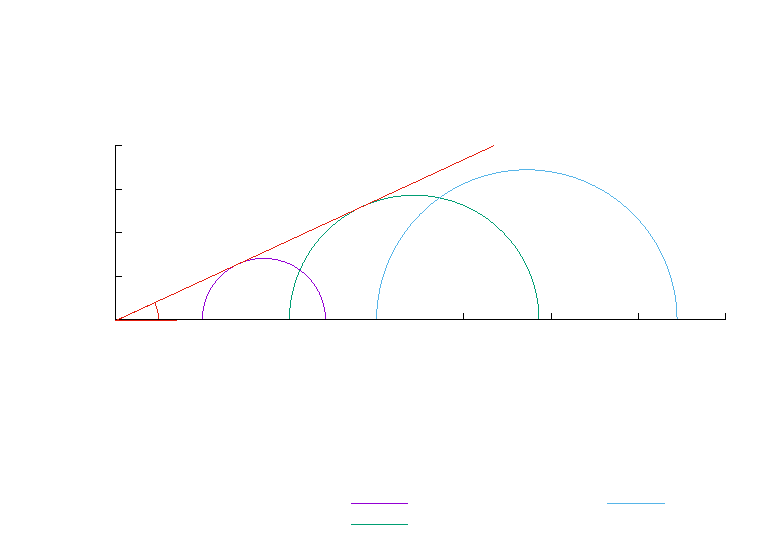
\includegraphics[width={360.00bp},height={252.00bp}]{./Cohesion_Critique}}%
    \gplfronttext
  \end{picture}%
\endgroup
}
        \caption{À l’état critique}
        \label{fig:muresiduel}
    \end{subfigure}
    \hfill
    \begin{subfigure}[b]{0.49\textwidth}
        \centering \small
        \scalebox{0.5}{% GNUPLOT: LaTeX picture with Postscript
\begingroup
  \makeatletter
  \providecommand\color[2][]{%
    \GenericError{(gnuplot) \space\space\space\@spaces}{%
      Package color not loaded in conjunction with
      terminal option `colourtext'%
    }{See the gnuplot documentation for explanation.%
    }{Either use 'blacktext' in gnuplot or load the package
      color.sty in LaTeX.}%
    \renewcommand\color[2][]{}%
  }%
  \providecommand\includegraphics[2][]{%
    \GenericError{(gnuplot) \space\space\space\@spaces}{%
      Package graphicx or graphics not loaded%
    }{See the gnuplot documentation for explanation.%
    }{The gnuplot epslatex terminal needs graphicx.sty or graphics.sty.}%
    \renewcommand\includegraphics[2][]{}%
  }%
  \providecommand\rotatebox[2]{#2}%
  \@ifundefined{ifGPcolor}{%
    \newif\ifGPcolor
    \GPcolortrue
  }{}%
  \@ifundefined{ifGPblacktext}{%
    \newif\ifGPblacktext
    \GPblacktextfalse
  }{}%
  % define a \g@addto@macro without @ in the name:
  \let\gplgaddtomacro\g@addto@macro
  % define empty templates for all commands taking text:
  \gdef\gplbacktext{}%
  \gdef\gplfronttext{}%
  \makeatother
  \ifGPblacktext
    % no textcolor at all
    \def\colorrgb#1{}%
    \def\colorgray#1{}%
  \else
    % gray or color?
    \ifGPcolor
      \def\colorrgb#1{\color[rgb]{#1}}%
      \def\colorgray#1{\color[gray]{#1}}%
      \expandafter\def\csname LTw\endcsname{\color{white}}%
      \expandafter\def\csname LTb\endcsname{\color{black}}%
      \expandafter\def\csname LTa\endcsname{\color{black}}%
      \expandafter\def\csname LT0\endcsname{\color[rgb]{1,0,0}}%
      \expandafter\def\csname LT1\endcsname{\color[rgb]{0,1,0}}%
      \expandafter\def\csname LT2\endcsname{\color[rgb]{0,0,1}}%
      \expandafter\def\csname LT3\endcsname{\color[rgb]{1,0,1}}%
      \expandafter\def\csname LT4\endcsname{\color[rgb]{0,1,1}}%
      \expandafter\def\csname LT5\endcsname{\color[rgb]{1,1,0}}%
      \expandafter\def\csname LT6\endcsname{\color[rgb]{0,0,0}}%
      \expandafter\def\csname LT7\endcsname{\color[rgb]{1,0.3,0}}%
      \expandafter\def\csname LT8\endcsname{\color[rgb]{0.5,0.5,0.5}}%
    \else
      % gray
      \def\colorrgb#1{\color{black}}%
      \def\colorgray#1{\color[gray]{#1}}%
      \expandafter\def\csname LTw\endcsname{\color{white}}%
      \expandafter\def\csname LTb\endcsname{\color{black}}%
      \expandafter\def\csname LTa\endcsname{\color{black}}%
      \expandafter\def\csname LT0\endcsname{\color{black}}%
      \expandafter\def\csname LT1\endcsname{\color{black}}%
      \expandafter\def\csname LT2\endcsname{\color{black}}%
      \expandafter\def\csname LT3\endcsname{\color{black}}%
      \expandafter\def\csname LT4\endcsname{\color{black}}%
      \expandafter\def\csname LT5\endcsname{\color{black}}%
      \expandafter\def\csname LT6\endcsname{\color{black}}%
      \expandafter\def\csname LT7\endcsname{\color{black}}%
      \expandafter\def\csname LT8\endcsname{\color{black}}%
    \fi
  \fi
    \setlength{\unitlength}{0.0500bp}%
    \ifx\gptboxheight\undefined%
      \newlength{\gptboxheight}%
      \newlength{\gptboxwidth}%
      \newsavebox{\gptboxtext}%
    \fi%
    \setlength{\fboxrule}{0.5pt}%
    \setlength{\fboxsep}{1pt}%
    \definecolor{tbcol}{rgb}{1,1,1}%
\begin{picture}(7200.00,5040.00)%
    \gplgaddtomacro\gplbacktext{%
      \csname LTb\endcsname%%
      \put(814,1506){\makebox(0,0)[r]{\strut{}$0$}}%
      \put(814,1925){\makebox(0,0)[r]{\strut{}$100$}}%
      \put(814,2343){\makebox(0,0)[r]{\strut{}$200$}}%
      \put(814,2762){\makebox(0,0)[r]{\strut{}$300$}}%
      \put(814,3180){\makebox(0,0)[r]{\strut{}$400$}}%
      \put(814,3599){\makebox(0,0)[r]{\strut{}$500$}}%
      \put(814,4017){\makebox(0,0)[r]{\strut{}$600$}}%
      \put(946,1286){\makebox(0,0){\strut{}$0$}}%
      \put(1783,1286){\makebox(0,0){\strut{}$200$}}%
      \put(2619,1286){\makebox(0,0){\strut{}$400$}}%
      \put(3456,1286){\makebox(0,0){\strut{}$600$}}%
      \put(4293,1286){\makebox(0,0){\strut{}$800$}}%
      \put(5130,1286){\makebox(0,0){\strut{}$1000$}}%
      \put(5966,1286){\makebox(0,0){\strut{}$1200$}}%
      \put(6803,1286){\makebox(0,0){\strut{}$1400$}}%
      \colorrgb{0.90,0.12,0.06}%%
      \put(1323,2119){\makebox(0,0)[l]{\strut{}$\varphi = 30.58^\circ$}}%
      \put(1113,1851){\makebox(0,0)[l]{\strut{}c = 122.44^}}%
    }%
    \gplgaddtomacro\gplfronttext{%
      \csname LTb\endcsname%%
      \put(209,2761){\rotatebox{-270}{\makebox(0,0){\strut{}$\tau$ (kPa)}}}%
      \put(3874,956){\makebox(0,0){\strut{}$\sigma_n$ (kPa)}}%
    }%
    \gplbacktext
    \put(0,0){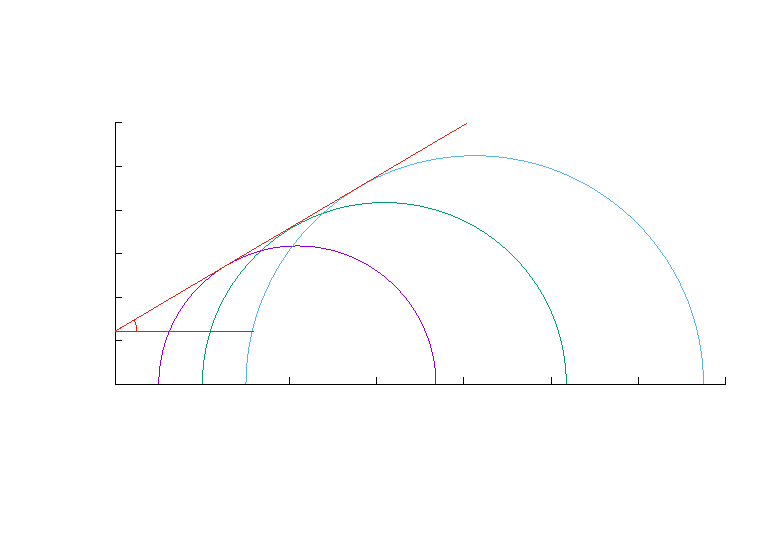
\includegraphics[width={360.00bp},height={252.00bp}]{Cohesion}}%
    \gplfronttext
  \end{picture}%
\endgroup
}
        \caption{Au pic}
        \label{fig:mutransitore}
    \end{subfigure}
    \caption{Cercle de Mohr d’un échantillon dense quand $I \approx 10^{-2}$}
    \label{fig:CercleDuMohrRapide}
\end{figure}

Malheureusement, bien que les tangentes aux cercles de Mohr se confondent, la cohésion selon la condition de Mohr (figure \ref{fig:CercleDuMohrRapide}) au pic n’est pas nulle.  
Cela constitue un verrou identifié dans la thèse, lié à un problème des conditions aux limites périodiques. Ce problème est actuellement en cours de résolution.  
Entre-temps, l’état critique donne une cohésion proche de zéro ($c \approx 0$), ce qui nous permet d’utiliser la rhéologie $\mu(I)$ afin de préparer le couplage avec le modèle d’écoulement.

\section{Rhéologie $\mu(I)$ résiduelle}

La rhéologie $\mu(I)$ joue un rôle crucial dans la description des écoulements granulaires. Elle établit une relation constitutive entre le tenseur des contraintes du flux et le tenseur des taux de déformation~\citep{jop2006constitutive} :
\begin{equation}
\sigma_{ij} = -P \delta_{ij} + \mu(I) P \frac{\dot{\gamma}_{ij}}{\lVert \dot{\gamma} \rVert}
\label{flowTensor}
\end{equation}
où :
\begin{equation}
\mu(I) = \mu_s + \dfrac{\mu_2 - \mu_s}{1 + \dfrac{I_0}{I}}
\label{muI}
\end{equation}
\begin{equation}
\Phi(I) = \Phi^{\max} - bI
\label{phiI}
\end{equation}

\begin{equation}
I =  \frac{\dot{\varepsilon} \cdot \bar{a}}{\sqrt{\sigma_{33}/\rho_s}}
\label{IMacro}
\end{equation}

Les coefficients $\mu_s$, $\mu_2$, $I_0$, $\Phi_{\max}$, et $b$ sont déterminés empiriquement.

\begin{figure}[h!]
    \centering
    \subfloat[Contrainte–Déformation]{\scalebox{0.49}{\small % GNUPLOT: LaTeX picture with Postscript
\begingroup
  \makeatletter
  \providecommand\color[2][]{%
    \GenericError{(gnuplot) \space\space\space\@spaces}{%
      Package color not loaded in conjunction with
      terminal option `colourtext'%
    }{See the gnuplot documentation for explanation.%
    }{Either use 'blacktext' in gnuplot or load the package
      color.sty in LaTeX.}%
    \renewcommand\color[2][]{}%
  }%
  \providecommand\includegraphics[2][]{%
    \GenericError{(gnuplot) \space\space\space\@spaces}{%
      Package graphicx or graphics not loaded%
    }{See the gnuplot documentation for explanation.%
    }{The gnuplot epslatex terminal needs graphicx.sty or graphics.sty.}%
    \renewcommand\includegraphics[2][]{}%
  }%
  \providecommand\rotatebox[2]{#2}%
  \@ifundefined{ifGPcolor}{%
    \newif\ifGPcolor
    \GPcolortrue
  }{}%
  \@ifundefined{ifGPblacktext}{%
    \newif\ifGPblacktext
    \GPblacktextfalse
  }{}%
  % define a \g@addto@macro without @ in the name:
  \let\gplgaddtomacro\g@addto@macro
  % define empty templates for all commands taking text:
  \gdef\gplbacktext{}%
  \gdef\gplfronttext{}%
  \makeatother
  \ifGPblacktext
    % no textcolor at all
    \def\colorrgb#1{}%
    \def\colorgray#1{}%
  \else
    % gray or color?
    \ifGPcolor
      \def\colorrgb#1{\color[rgb]{#1}}%
      \def\colorgray#1{\color[gray]{#1}}%
      \expandafter\def\csname LTw\endcsname{\color{white}}%
      \expandafter\def\csname LTb\endcsname{\color{black}}%
      \expandafter\def\csname LTa\endcsname{\color{black}}%
      \expandafter\def\csname LT0\endcsname{\color[rgb]{1,0,0}}%
      \expandafter\def\csname LT1\endcsname{\color[rgb]{0,1,0}}%
      \expandafter\def\csname LT2\endcsname{\color[rgb]{0,0,1}}%
      \expandafter\def\csname LT3\endcsname{\color[rgb]{1,0,1}}%
      \expandafter\def\csname LT4\endcsname{\color[rgb]{0,1,1}}%
      \expandafter\def\csname LT5\endcsname{\color[rgb]{1,1,0}}%
      \expandafter\def\csname LT6\endcsname{\color[rgb]{0,0,0}}%
      \expandafter\def\csname LT7\endcsname{\color[rgb]{1,0.3,0}}%
      \expandafter\def\csname LT8\endcsname{\color[rgb]{0.5,0.5,0.5}}%
    \else
      % gray
      \def\colorrgb#1{\color{black}}%
      \def\colorgray#1{\color[gray]{#1}}%
      \expandafter\def\csname LTw\endcsname{\color{white}}%
      \expandafter\def\csname LTb\endcsname{\color{black}}%
      \expandafter\def\csname LTa\endcsname{\color{black}}%
      \expandafter\def\csname LT0\endcsname{\color{black}}%
      \expandafter\def\csname LT1\endcsname{\color{black}}%
      \expandafter\def\csname LT2\endcsname{\color{black}}%
      \expandafter\def\csname LT3\endcsname{\color{black}}%
      \expandafter\def\csname LT4\endcsname{\color{black}}%
      \expandafter\def\csname LT5\endcsname{\color{black}}%
      \expandafter\def\csname LT6\endcsname{\color{black}}%
      \expandafter\def\csname LT7\endcsname{\color{black}}%
      \expandafter\def\csname LT8\endcsname{\color{black}}%
    \fi
  \fi
    \setlength{\unitlength}{0.0500bp}%
    \ifx\gptboxheight\undefined%
      \newlength{\gptboxheight}%
      \newlength{\gptboxwidth}%
      \newsavebox{\gptboxtext}%
    \fi%
    \setlength{\fboxrule}{0.5pt}%
    \setlength{\fboxsep}{1pt}%
    \definecolor{tbcol}{rgb}{1,1,1}%
\begin{picture}(7200.00,5040.00)%
    \gplgaddtomacro\gplbacktext{%
      \csname LTb\endcsname%%
      \put(946,1584){\makebox(0,0)[r]{\strut{}$0$}}%
      \csname LTb\endcsname%%
      \put(946,2123){\makebox(0,0)[r]{\strut{}$200$}}%
      \csname LTb\endcsname%%
      \put(946,2662){\makebox(0,0)[r]{\strut{}$400$}}%
      \csname LTb\endcsname%%
      \put(946,3202){\makebox(0,0)[r]{\strut{}$600$}}%
      \csname LTb\endcsname%%
      \put(946,3741){\makebox(0,0)[r]{\strut{}$800$}}%
      \csname LTb\endcsname%%
      \put(946,4280){\makebox(0,0)[r]{\strut{}$1000$}}%
      \csname LTb\endcsname%%
      \put(946,4819){\makebox(0,0)[r]{\strut{}$1200$}}%
      \csname LTb\endcsname%%
      \put(1078,1364){\makebox(0,0){\strut{}$0$}}%
      \csname LTb\endcsname%%
      \put(1700,1364){\makebox(0,0){\strut{}$10$}}%
      \csname LTb\endcsname%%
      \put(2322,1364){\makebox(0,0){\strut{}$20$}}%
      \csname LTb\endcsname%%
      \put(2944,1364){\makebox(0,0){\strut{}$30$}}%
      \csname LTb\endcsname%%
      \put(3567,1364){\makebox(0,0){\strut{}$40$}}%
      \csname LTb\endcsname%%
      \put(4189,1364){\makebox(0,0){\strut{}$50$}}%
      \csname LTb\endcsname%%
      \put(4811,1364){\makebox(0,0){\strut{}$60$}}%
      \csname LTb\endcsname%%
      \put(5433,1364){\makebox(0,0){\strut{}$70$}}%
      \csname LTb\endcsname%%
      \put(6055,1364){\makebox(0,0){\strut{}$80$}}%
      \put(6187,1584){\makebox(0,0)[l]{\strut{}$-2$}}%
      \put(6187,1908){\makebox(0,0)[l]{\strut{}$-1$}}%
      \put(6187,2231){\makebox(0,0)[l]{\strut{}$0$}}%
      \put(6187,2555){\makebox(0,0)[l]{\strut{}$1$}}%
      \put(6187,2878){\makebox(0,0)[l]{\strut{}$2$}}%
      \put(6187,3202){\makebox(0,0)[l]{\strut{}$3$}}%
      \put(6187,3525){\makebox(0,0)[l]{\strut{}$4$}}%
      \put(6187,3849){\makebox(0,0)[l]{\strut{}$5$}}%
      \put(6187,4172){\makebox(0,0)[l]{\strut{}$6$}}%
      \put(6187,4496){\makebox(0,0)[l]{\strut{}$7$}}%
      \put(6187,4819){\makebox(0,0)[l]{\strut{}$8$}}%
    }%
    \gplgaddtomacro\gplfronttext{%
      \csname LTb\endcsname%%
      \put(341,3201){\rotatebox{-270}{\makebox(0,0){\strut{}q (kPa)}}}%
      \put(6693,3201){\rotatebox{-270}{\makebox(0,0){\strut{}$\varepsilon_v$ (\%)}}}%
      \put(3566,1034){\makebox(0,0){\strut{}$\varepsilon_{yy}$ (\%)}}%
      \csname LTb\endcsname%%
      \put(2711,833){\makebox(0,0)[r]{\strut{}$I = 1 \times 10^{-4}$}}%
      \csname LTb\endcsname%%
      \put(2711,613){\makebox(0,0)[r]{\strut{}$I = 1 \times 10^{-3}$}}%
      \csname LTb\endcsname%%
      \put(2711,393){\makebox(0,0)[r]{\strut{}$I = 2 \times 10^{-3}$}}%
      \csname LTb\endcsname%%
      \put(2711,173){\makebox(0,0)[r]{\strut{}$I = 4 \times 10^{-3}$}}%
      \csname LTb\endcsname%%
      \put(5150,833){\makebox(0,0)[r]{\strut{}$I = 6 \times 10^{-3}$}}%
      \csname LTb\endcsname%%
      \put(5150,613){\makebox(0,0)[r]{\strut{}$I = 8 \times 10^{-3}$}}%
      \csname LTb\endcsname%%
      \put(5150,393){\makebox(0,0)[r]{\strut{}$I = 1 \times 10^{-2}$}}%
    }%
    \gplbacktext
    \put(0,0){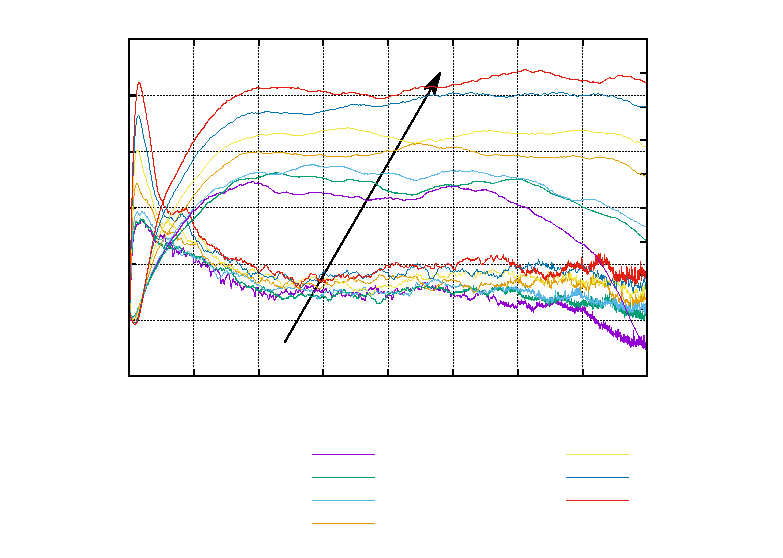
\includegraphics[width={360.00bp},height={252.00bp}]{./Test}}%
    \gplfronttext
  \end{picture}%
\endgroup
}\label{fig:etudeSurI1}}
    \subfloat[Cercles résiduels]{\scalebox{0.49}{\small \input{Résiduel.tex}}\label{fig:cercleResiduel1}}
  \caption{Influence du nombre d’inertie sur la condition de Mohr-Coulomb}
  \label{fig:IResiduel}
\end{figure}

\begin{figure}[h!]
    \centering
    \subfloat[$\mu(I)$]{\scalebox{0.49}{\small % GNUPLOT: LaTeX picture with Postscript
\begingroup
  \makeatletter
  \providecommand\color[2][]{%
    \GenericError{(gnuplot) \space\space\space\@spaces}{%
      Package color not loaded in conjunction with
      terminal option `colourtext'%
    }{See the gnuplot documentation for explanation.%
    }{Either use 'blacktext' in gnuplot or load the package
      color.sty in LaTeX.}%
    \renewcommand\color[2][]{}%
  }%
  \providecommand\includegraphics[2][]{%
    \GenericError{(gnuplot) \space\space\space\@spaces}{%
      Package graphicx or graphics not loaded%
    }{See the gnuplot documentation for explanation.%
    }{The gnuplot epslatex terminal needs graphicx.sty or graphics.sty.}%
    \renewcommand\includegraphics[2][]{}%
  }%
  \providecommand\rotatebox[2]{#2}%
  \@ifundefined{ifGPcolor}{%
    \newif\ifGPcolor
    \GPcolortrue
  }{}%
  \@ifundefined{ifGPblacktext}{%
    \newif\ifGPblacktext
    \GPblacktextfalse
  }{}%
  % define a \g@addto@macro without @ in the name:
  \let\gplgaddtomacro\g@addto@macro
  % define empty templates for all commands taking text:
  \gdef\gplbacktext{}%
  \gdef\gplfronttext{}%
  \makeatother
  \ifGPblacktext
    % no textcolor at all
    \def\colorrgb#1{}%
    \def\colorgray#1{}%
  \else
    % gray or color?
    \ifGPcolor
      \def\colorrgb#1{\color[rgb]{#1}}%
      \def\colorgray#1{\color[gray]{#1}}%
      \expandafter\def\csname LTw\endcsname{\color{white}}%
      \expandafter\def\csname LTb\endcsname{\color{black}}%
      \expandafter\def\csname LTa\endcsname{\color{black}}%
      \expandafter\def\csname LT0\endcsname{\color[rgb]{1,0,0}}%
      \expandafter\def\csname LT1\endcsname{\color[rgb]{0,1,0}}%
      \expandafter\def\csname LT2\endcsname{\color[rgb]{0,0,1}}%
      \expandafter\def\csname LT3\endcsname{\color[rgb]{1,0,1}}%
      \expandafter\def\csname LT4\endcsname{\color[rgb]{0,1,1}}%
      \expandafter\def\csname LT5\endcsname{\color[rgb]{1,1,0}}%
      \expandafter\def\csname LT6\endcsname{\color[rgb]{0,0,0}}%
      \expandafter\def\csname LT7\endcsname{\color[rgb]{1,0.3,0}}%
      \expandafter\def\csname LT8\endcsname{\color[rgb]{0.5,0.5,0.5}}%
    \else
      % gray
      \def\colorrgb#1{\color{black}}%
      \def\colorgray#1{\color[gray]{#1}}%
      \expandafter\def\csname LTw\endcsname{\color{white}}%
      \expandafter\def\csname LTb\endcsname{\color{black}}%
      \expandafter\def\csname LTa\endcsname{\color{black}}%
      \expandafter\def\csname LT0\endcsname{\color{black}}%
      \expandafter\def\csname LT1\endcsname{\color{black}}%
      \expandafter\def\csname LT2\endcsname{\color{black}}%
      \expandafter\def\csname LT3\endcsname{\color{black}}%
      \expandafter\def\csname LT4\endcsname{\color{black}}%
      \expandafter\def\csname LT5\endcsname{\color{black}}%
      \expandafter\def\csname LT6\endcsname{\color{black}}%
      \expandafter\def\csname LT7\endcsname{\color{black}}%
      \expandafter\def\csname LT8\endcsname{\color{black}}%
    \fi
  \fi
    \setlength{\unitlength}{0.0500bp}%
    \ifx\gptboxheight\undefined%
      \newlength{\gptboxheight}%
      \newlength{\gptboxwidth}%
      \newsavebox{\gptboxtext}%
    \fi%
    \setlength{\fboxrule}{0.5pt}%
    \setlength{\fboxsep}{1pt}%
    \definecolor{tbcol}{rgb}{1,1,1}%
\begin{picture}(7200.00,5040.00)%
    \gplgaddtomacro\gplbacktext{%
      \csname LTb\endcsname%%
      \put(946,704){\makebox(0,0)[r]{\strut{}$0.28$}}%
      \csname LTb\endcsname%%
      \put(946,1161){\makebox(0,0)[r]{\strut{}$0.3$}}%
      \csname LTb\endcsname%%
      \put(946,1618){\makebox(0,0)[r]{\strut{}$0.32$}}%
      \csname LTb\endcsname%%
      \put(946,2076){\makebox(0,0)[r]{\strut{}$0.34$}}%
      \csname LTb\endcsname%%
      \put(946,2533){\makebox(0,0)[r]{\strut{}$0.36$}}%
      \csname LTb\endcsname%%
      \put(946,2990){\makebox(0,0)[r]{\strut{}$0.38$}}%
      \csname LTb\endcsname%%
      \put(946,3447){\makebox(0,0)[r]{\strut{}$0.4$}}%
      \csname LTb\endcsname%%
      \put(946,3905){\makebox(0,0)[r]{\strut{}$0.42$}}%
      \csname LTb\endcsname%%
      \put(946,4362){\makebox(0,0)[r]{\strut{}$0.44$}}%
      \csname LTb\endcsname%%
      \put(946,4819){\makebox(0,0)[r]{\strut{}$0.46$}}%
      \csname LTb\endcsname%%
      \put(1078,484){\makebox(0,0){\strut{}$10^{-4}$}}%
      \csname LTb\endcsname%%
      \put(2986,484){\makebox(0,0){\strut{}$10^{-3}$}}%
      \csname LTb\endcsname%%
      \put(4895,484){\makebox(0,0){\strut{}$10^{-2}$}}%
      \csname LTb\endcsname%%
      \put(6803,484){\makebox(0,0){\strut{}$10^{-1}$}}%
      \put(1651,3996){\makebox(0,0)[l]{\strut{}$\mu_s = 0.2953$}}%
      \put(1651,3585){\makebox(0,0)[l]{\strut{}$\mu_2 = 0.5329$}}%
      \put(1651,3173){\makebox(0,0)[l]{\strut{}$I_0 = 0.0483$}}%
    }%
    \gplgaddtomacro\gplfronttext{%
      \csname LTb\endcsname%%
      \put(209,2761){\rotatebox{-270}{\makebox(0,0){\strut{}$\mu$}}}%
      \put(3940,154){\makebox(0,0){\strut{}$I$}}%
      \csname LTb\endcsname%%
      \put(3322,4646){\makebox(0,0)[r]{\strut{}Données}}%
      \csname LTb\endcsname%%
      \put(3322,4426){\makebox(0,0)[r]{\strut{}$\mu(I)$ régression}}%
    }%
    \gplbacktext
    \put(0,0){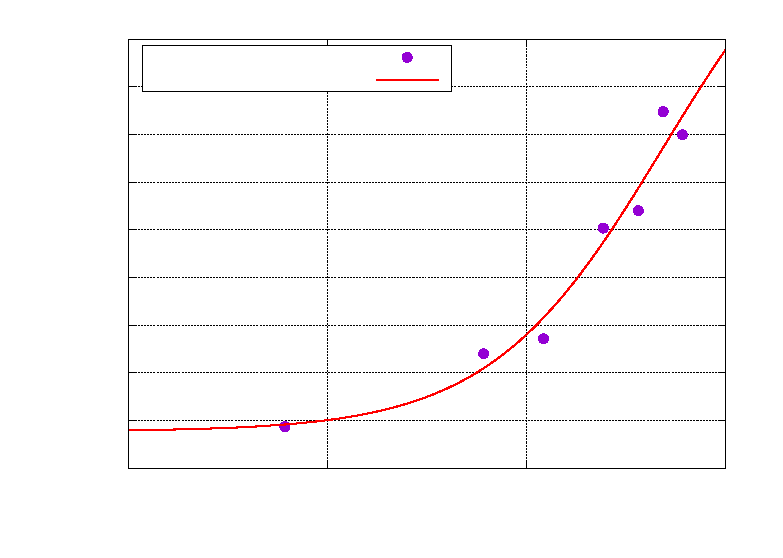
\includegraphics[width={360.00bp},height={252.00bp}]{./mu_I_fit}}%
    \gplfronttext
  \end{picture}%
\endgroup
}\label{fig:etudeSurI2}}
    \subfloat[$\Phi(I)$]{\scalebox{0.49}{\small % GNUPLOT: LaTeX picture with Postscript
\begingroup
  \makeatletter
  \providecommand\color[2][]{%
    \GenericError{(gnuplot) \space\space\space\@spaces}{%
      Package color not loaded in conjunction with
      terminal option `colourtext'%
    }{See the gnuplot documentation for explanation.%
    }{Either use 'blacktext' in gnuplot or load the package
      color.sty in LaTeX.}%
    \renewcommand\color[2][]{}%
  }%
  \providecommand\includegraphics[2][]{%
    \GenericError{(gnuplot) \space\space\space\@spaces}{%
      Package graphicx or graphics not loaded%
    }{See the gnuplot documentation for explanation.%
    }{The gnuplot epslatex terminal needs graphicx.sty or graphics.sty.}%
    \renewcommand\includegraphics[2][]{}%
  }%
  \providecommand\rotatebox[2]{#2}%
  \@ifundefined{ifGPcolor}{%
    \newif\ifGPcolor
    \GPcolortrue
  }{}%
  \@ifundefined{ifGPblacktext}{%
    \newif\ifGPblacktext
    \GPblacktextfalse
  }{}%
  % define a \g@addto@macro without @ in the name:
  \let\gplgaddtomacro\g@addto@macro
  % define empty templates for all commands taking text:
  \gdef\gplbacktext{}%
  \gdef\gplfronttext{}%
  \makeatother
  \ifGPblacktext
    % no textcolor at all
    \def\colorrgb#1{}%
    \def\colorgray#1{}%
  \else
    % gray or color?
    \ifGPcolor
      \def\colorrgb#1{\color[rgb]{#1}}%
      \def\colorgray#1{\color[gray]{#1}}%
      \expandafter\def\csname LTw\endcsname{\color{white}}%
      \expandafter\def\csname LTb\endcsname{\color{black}}%
      \expandafter\def\csname LTa\endcsname{\color{black}}%
      \expandafter\def\csname LT0\endcsname{\color[rgb]{1,0,0}}%
      \expandafter\def\csname LT1\endcsname{\color[rgb]{0,1,0}}%
      \expandafter\def\csname LT2\endcsname{\color[rgb]{0,0,1}}%
      \expandafter\def\csname LT3\endcsname{\color[rgb]{1,0,1}}%
      \expandafter\def\csname LT4\endcsname{\color[rgb]{0,1,1}}%
      \expandafter\def\csname LT5\endcsname{\color[rgb]{1,1,0}}%
      \expandafter\def\csname LT6\endcsname{\color[rgb]{0,0,0}}%
      \expandafter\def\csname LT7\endcsname{\color[rgb]{1,0.3,0}}%
      \expandafter\def\csname LT8\endcsname{\color[rgb]{0.5,0.5,0.5}}%
    \else
      % gray
      \def\colorrgb#1{\color{black}}%
      \def\colorgray#1{\color[gray]{#1}}%
      \expandafter\def\csname LTw\endcsname{\color{white}}%
      \expandafter\def\csname LTb\endcsname{\color{black}}%
      \expandafter\def\csname LTa\endcsname{\color{black}}%
      \expandafter\def\csname LT0\endcsname{\color{black}}%
      \expandafter\def\csname LT1\endcsname{\color{black}}%
      \expandafter\def\csname LT2\endcsname{\color{black}}%
      \expandafter\def\csname LT3\endcsname{\color{black}}%
      \expandafter\def\csname LT4\endcsname{\color{black}}%
      \expandafter\def\csname LT5\endcsname{\color{black}}%
      \expandafter\def\csname LT6\endcsname{\color{black}}%
      \expandafter\def\csname LT7\endcsname{\color{black}}%
      \expandafter\def\csname LT8\endcsname{\color{black}}%
    \fi
  \fi
    \setlength{\unitlength}{0.0500bp}%
    \ifx\gptboxheight\undefined%
      \newlength{\gptboxheight}%
      \newlength{\gptboxwidth}%
      \newsavebox{\gptboxtext}%
    \fi%
    \setlength{\fboxrule}{0.5pt}%
    \setlength{\fboxsep}{1pt}%
    \definecolor{tbcol}{rgb}{1,1,1}%
\begin{picture}(7200.00,5040.00)%
    \gplgaddtomacro\gplbacktext{%
      \csname LTb\endcsname%%
      \put(1078,704){\makebox(0,0)[r]{\strut{}$0.555$}}%
      \csname LTb\endcsname%%
      \put(1078,1116){\makebox(0,0)[r]{\strut{}$0.56$}}%
      \csname LTb\endcsname%%
      \put(1078,1527){\makebox(0,0)[r]{\strut{}$0.565$}}%
      \csname LTb\endcsname%%
      \put(1078,1939){\makebox(0,0)[r]{\strut{}$0.57$}}%
      \csname LTb\endcsname%%
      \put(1078,2350){\makebox(0,0)[r]{\strut{}$0.575$}}%
      \csname LTb\endcsname%%
      \put(1078,2762){\makebox(0,0)[r]{\strut{}$0.58$}}%
      \csname LTb\endcsname%%
      \put(1078,3173){\makebox(0,0)[r]{\strut{}$0.585$}}%
      \csname LTb\endcsname%%
      \put(1078,3585){\makebox(0,0)[r]{\strut{}$0.59$}}%
      \csname LTb\endcsname%%
      \put(1078,3996){\makebox(0,0)[r]{\strut{}$0.595$}}%
      \csname LTb\endcsname%%
      \put(1078,4408){\makebox(0,0)[r]{\strut{}$0.6$}}%
      \csname LTb\endcsname%%
      \put(1078,4819){\makebox(0,0)[r]{\strut{}$0.605$}}%
      \csname LTb\endcsname%%
      \put(1210,484){\makebox(0,0){\strut{}$10^{-4}$}}%
      \csname LTb\endcsname%%
      \put(3074,484){\makebox(0,0){\strut{}$10^{-3}$}}%
      \csname LTb\endcsname%%
      \put(4939,484){\makebox(0,0){\strut{}$10^{-2}$}}%
      \csname LTb\endcsname%%
      \put(6803,484){\makebox(0,0){\strut{}$10^{-1}$}}%
      \put(1769,1733){\makebox(0,0)[l]{\strut{}$\Phi_{max} = 0.6019$}}%
      \put(1769,1321){\makebox(0,0)[l]{\strut{}$b = 0.4641$}}%
    }%
    \gplgaddtomacro\gplfronttext{%
      \csname LTb\endcsname%%
      \put(209,2761){\rotatebox{-270}{\makebox(0,0){\strut{}$\Phi$}}}%
      \put(4006,154){\makebox(0,0){\strut{}$I$}}%
      \csname LTb\endcsname%%
      \put(3454,1097){\makebox(0,0)[r]{\strut{}Données}}%
      \csname LTb\endcsname%%
      \put(3454,877){\makebox(0,0)[r]{\strut{}$\Phi(I)$ régression}}%
    }%
    \gplbacktext
    \put(0,0){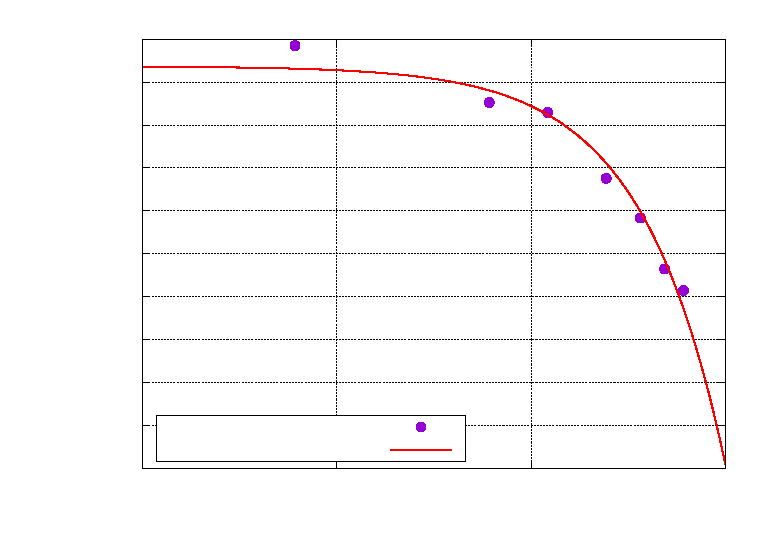
\includegraphics[width={360.00bp},height={252.00bp}]{./Pack_I_fit}}%
    \gplfronttext
  \end{picture}%
\endgroup
}\label{fig:cercleResiduel2}}
  \caption{Étude de la rhéologie à l’état critique}
  \label{fig:Rheologie}
\end{figure}

La petite plage de l’axe des ordonnées de la figure~\ref{fig:Rheologie} indique que les valeurs suivent une tendance cohérente.

\chapter{Conclusion}

Au cours de ma première année de thèse, j’ai eu l’opportunité de me familiariser avec des méthodes numériques avancées telles que la Méthode des Éléments Discrets (DEM) et la Méthode des Points Matériels (MPM).  
Sous la direction du Professeur Gaël COMBE, du MCF-HDR Vincent RICHEFEU du laboratoire 3SR, Université Grenoble Alpes, et plus récemment du Professeur Associé Trung Kien NGUYEN de l’École de Génie Civil de Hanoi, j’ai acquis des connaissances fondamentales sur la modélisation des matériaux granulaires, notamment à travers l’étude des essais triaxiaux et l’implémentation des algorithmes DEM/MPM dans des codes numériques.

L’encadrement rigoureux de mes directeurs de thèse m’a permis d’approfondir ma compréhension des problématiques classiques des milieux granulaires et d’accéder à une documentation scientifique de qualité. Par ailleurs, j’ai pu développer mes compétences en programmation (C++), en rédaction scientifique (LaTeX) et en visualisation de données (Gnuplot), outils essentiels pour la conduite de simulations numériques et l’analyse des résultats.

Les travaux réalisés ont validé la robustesse des outils numériques développés, notamment dans le cadre de simulations quasi-statiques. Cependant, certaines limitations persistent, notamment en ce qui concerne la gestion des conditions aux limites dans le couplage MPM-DEM, qui demeure un défi majeur pour la modélisation précise des écoulements granulaires dynamiques. Ce verrou scientifique a été clairement identifié et fait l’objet de développements méthodologiques en cours.

Les perspectives pour la suite de la thèse incluent l’amélioration du couplage entre les deux codes, l’intégration des lois de comportement adaptées à l’état critique, ainsi que la réalisation de simulations à plus grande échelle afin de mieux représenter les phénomènes naturels étudiés.
Je tiens à exprimer ma profonde gratitude à mes encadrants pour leur soutien constant et leurs conseils avisés. Enfin, je reste attentif aux remarques et suggestions du comité du CSI, qui seront précieux pour la poursuite et la réussite de ce travail de recherche.

\bibliographystyle{apalike}
\bibliography{Bibliographie}

\end{document}


